\documentclass{article}
\usepackage[preprint]{neurips_2024}

\usepackage[utf8]{inputenc}
\usepackage[T1]{fontenc}
\usepackage{amsmath,amssymb}
\usepackage{graphicx}
\usepackage{booktabs}
\usepackage{hyperref}
\usepackage{url}
\usepackage{algorithm}
\usepackage{algorithmic}
\usepackage{microtype}
\usepackage{tikz}
\usetikzlibrary{positioning, arrows.meta, calc, fit, backgrounds, decorations.pathreplacing}

\graphicspath{{../experiment/paper_figures/}{../experiment_mossies/paper_figures/}{../experiment_mossies/data_application/results/}{../experiment-large-context/paper_figures/}}

\title{fastcxt: Linear-Scale Genome-Wide TMRCA Inference}

\author{
  Kevin Korfmann \\
  University of Pennsylvania
  \And
  Sara Mathieson \\
  University of Pennsylvania
}

\begin{document}
\maketitle

\begin{abstract}
Pairwise coalescence times (TMRCAs) along the genome encode rich information about
demographic history, natural selection, and population structure. Recently,
\texttt{cxt}~\citep{korfmann2025cxt} introduced a decoder-only transformer that treats TMRCA
inference as a language-modeling task---autoregressively predicting coalescence events from
local mutation patterns. While accurate and general, \texttt{cxt} inherits the $O(n^2)$
cost of pairwise methods: each of the $\binom{n}{2}$ sample pairs requires a separate
autoregressive decode. Here we present \textsc{fastcxt}, which replaces the autoregressive
transformer with a bidirectional Mamba state-space encoder--decoder that predicts posterior
mean and variance of log-TMRCA at every genomic window in a single non-autoregressive
forward pass, trained with Beta-NLL loss for calibrated heteroscedastic uncertainty.
A tree-augmented variant conditioning on tsinfer-inferred topology features achieves
$r = 0.887$ (RMSE\,=\,0.558), demonstrating viability without the true genealogy.
To break the $O(n^2)$ scaling barrier we further introduce a node-time model that predicts
all internal node times in one forward pass; pairwise TMRCAs are then recovered via $O(1)$
LCA lookups. For $n = 30$--$100$ the node-time model provides 7--11$\times$ speedup over
the pairwise Mamba baseline, with the advantage growing linearly in $n$. Where
\texttt{cxt} requires minutes for genome-wide inference, \textsc{fastcxt} completes the
same task in seconds. Applied to \emph{Anopheles gambiae} chromosome~2L from the Ag1000G
dataset, \textsc{fastcxt} resolves the 2La inversion and Rdl selective-sweep signatures,
with predictions closely matching independent \texttt{tsdate} estimates.
\end{abstract}

\section{Introduction}

The time to the most recent common ancestor (TMRCA) between pairs of haplotypes varies along
the genome, shaped by recombination, mutation, drift, and selection. This variation encodes a
detailed record of evolutionary history---recent coalescence signals demographic bottlenecks or
selective sweeps, while deeply divergent regions may reflect balancing selection or population
structure~\citep{schiffels2014inferring}. Accurate, window-level TMRCA estimates underpin
demographic inference~\citep{li2011inference}, introgression
detection~\citep{racimo2017signatures}, recombination-map
estimation~\citep{spence2019inference}, and sweep
localization~\citep{stern2019approximate}.

Classical TMRCA inference proceeds through the sequentially Markov coalescent
(SMC)~\citep{mcvean2005approximating, li2011inference} and its
extensions~\citep{terhorst2017robust, speidel2019method}, modeling the hidden genealogical
process as a Markov chain along the chromosome. While statistically principled, these methods
face two practical limitations: (i)~per-pair cost must be repeated for each of the
$\binom{n}{2}$ pairs in a sample, making whole-genome analysis prohibitively expensive for
even moderate sample sizes, and (ii)~they typically produce point estimates or discrete-state
posterior decodings without calibrated, continuous uncertainty.

Recently, \texttt{cxt}~\citep{korfmann2025cxt} reframed coalescence-time inference as a
language-modeling problem, training a decoder-only transformer to autoregressively predict
pairwise TMRCAs conditioned on local mutation patterns across the site frequency spectrum
(SFS). Trained on the \texttt{stdpopsim} catalog, \texttt{cxt} achieves competitive accuracy
with likelihood-based methods while producing calibrated approximate posteriors. However,
two bottlenecks limit its scalability: (i)~the autoregressive decode is inherently sequential
along the genome, making each per-pair inference slow, and (ii)~inference must be repeated
independently for each of the $\binom{n}{2}$ sample pairs, compounding the cost
quadratically.

\paragraph{Contributions.} Building directly on \texttt{cxt}, we make three contributions:
\begin{enumerate}
  \item \textbf{Mamba-based architecture.} We introduce \textsc{fastcxt}, which replaces the
    autoregressive transformer with a bidirectional
    Mamba~\citep{gu2024mamba, dao2024transformers} encoder--decoder. The non-autoregressive
    design processes all 500--2{,}000 windows in a single forward pass, capturing long-range
    genealogical correlations across 1\,Mb blocks. The architecture conditions on the
    log-mutation rate via FiLM~\citep{perez2018film} and outputs heteroscedastic Gaussian
    parameters trained with Beta-NLL loss~\citep{seitzer2022pitfalls}.
  \item \textbf{Tree topology augmentation.} Augmenting the SFS input with compact topology
    features (coalescent rank order, subtree sizes, split balance) from local trees provides
    complementary information. With tsinfer-inferred trees, the model achieves $r = 0.887$
    and RMSE\,$= 0.558$, establishing the viability of the full pipeline on empirical data.
  \item \textbf{$O(n)$ node-time inference.} We address the $O(n^2)$ pairwise bottleneck
    with a node-time model: a separate Mamba network that predicts all $n - 1$ internal node
    times in a single forward pass. Pairwise TMRCAs are recovered in $O(1)$ per pair via
    precomputed LCA tables~\citep{bender2000lca}. At $n = 100$ (4{,}950 pairs) this yields
    an $11\times$ speedup over the pairwise Mamba baseline, growing as $O(n)$.
    Together, \textsc{fastcxt} completes genome-wide inference in seconds where \texttt{cxt}
    requires minutes.
\end{enumerate}

\section{Background}

\paragraph{Coalescence and the TMRCA.}
Under the coalescent~\citep{kingman1982coalescent}, the genealogical history of $n$ haplotypes
at a single locus is a random binary tree whose lineages merge backward in time. The TMRCA of a
pair $(i,j)$ is the time at which their lineages first share a common ancestor. Along a
recombining chromosome the local tree changes at recombination breakpoints, so pairwise TMRCA
varies as a function of genomic position---a pattern commonly modeled as a hidden Markov model
(HMM)~\citep{li2011inference}.

\paragraph{Site frequency spectrum.}
For a focal pair $(i,j)$ drawn from $n$ haplotypes, we compute a two-channel SFS in each
genomic window: the \emph{xor} channel counts sites heterozygous in the pair (informative about
divergence), while the \emph{xnor} channel counts homozygous sites (informative about shared
background). Each channel is a vector in $\mathbb{R}^{n_\mathrm{samples}}$, yielding a
per-window input of shape $(2, n_\mathrm{samples})$.

\paragraph{State-space models and Mamba.}
Mamba~\citep{gu2024mamba} extends classical state-space models with input-dependent (selective)
parameterization, achieving linear complexity $O(L)$ in sequence length $L$ versus the
$O(L^2)$ cost of attention, while maintaining strong empirical performance on long sequences
in language modeling, genomics~\citep{schiff2024caduceus}, and time-series forecasting.

\section{Methods}

\subsection{Problem Formulation}

Given a genotype matrix $G \in \{0, 1\}^{n \times m}$, a focal pair $(i,j)$, and variant
positions, we predict the log-TMRCA $y_w = \log T_{ij}(w)$ at each of $W$ non-overlapping
windows of $\Delta$\,bp spanning a genomic block (e.g., $W{=}500$, $\Delta{=}2{,}000$\,bp
for 1\,Mb; or $W{=}2{,}000$, $\Delta{=}200$\,bp for 400\,kb). The model outputs per-window mean
$\hat{\mu}_w$ and variance $\hat{\sigma}^2_w$, parameterizing a heteroscedastic Gaussian.

\subsection{Architecture}

Figure~\ref{fig:architecture} provides an overview. The model follows an encoder--decoder
design built on bidirectional Mamba layers. Unlike the autoregressive \texttt{cxt}
transformer~\citep{korfmann2025cxt}, \textsc{fastcxt} processes the entire 500-window
sequence in parallel; predictions at each position attend to both upstream and downstream
genomic context.

\paragraph{Multi-scale convolutional stem.}
The windowed SFS $X \in \mathbb{R}^{2 \times W \times n_\mathrm{max}}$ is compressed along
the frequency axis, merged via a $1{\times}1$ convolution into 64 channels, then processed by
four parallel 1D convolutions ($k \in \{3, 11, 31, 63\}$) capturing SFS patterns from
single-window ($6$\,kb) to block-level ($126$\,kb) scales. Outputs are concatenated
($4 {\times} 64 = 256$ channels) and projected through a two-layer MLP to
$H^{(0)} \in \mathbb{R}^{W \times d}$, summed with a learnable positional embedding.

\paragraph{Tree topology encoder (optional).}
For each window, five normalized features per internal node---coalescent rank, min-leaf indices
of left/right subtrees, and subtree sizes---yield a vector of dimension
$5(n_\mathrm{max} {-} 1)$, projected to $d$ and added to $H^{(0)}$.

\paragraph{Bidirectional Mamba encoder.}
Six BiMamba blocks, each applying LayerNorm, running two Mamba2
modules~\citep{dao2024transformers} in opposite scan directions, concatenating and projecting
back to $d$ with a residual, followed by a feed-forward network ($d \to 4d \to d$, GELU,
dropout $p{=}0.1$). The per-sample log-mutation rate $\log\mu$ conditions the first and last
layers via FiLM~\citep{perez2018film}.

\paragraph{Decoder and output heads.}
Four BiMamba blocks with U-Net-style skip connections from the encoder. Two parallel MLPs
($d \to d/2 \to 1$) produce $\hat{\mu}_w$ and $\log\hat{\sigma}^2_w$.

\begin{figure}[t]
\centering
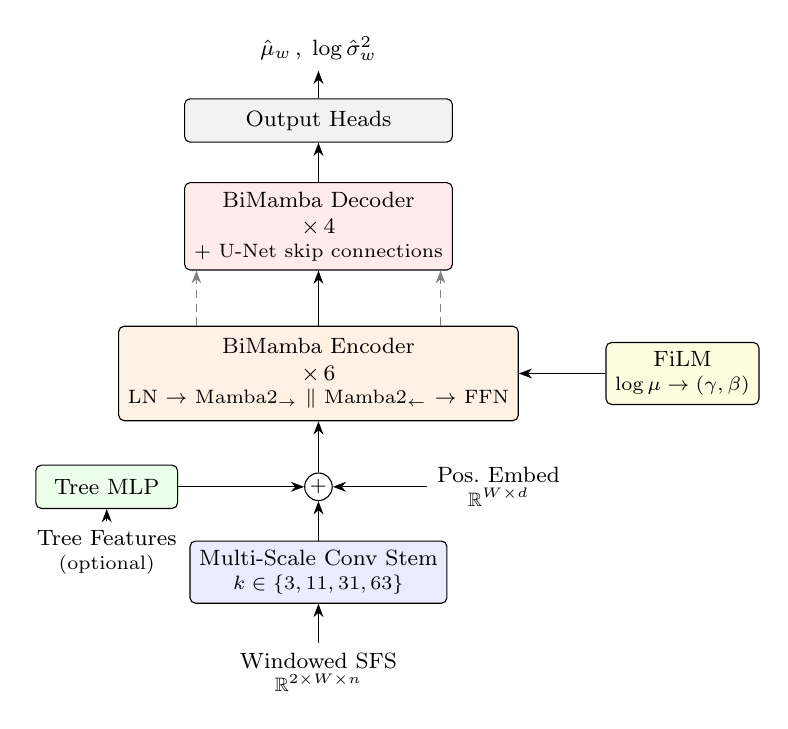
\begin{tikzpicture}[
    >=Stealth,
    node distance=0.6cm,
    block/.style={draw, rounded corners=2pt, minimum width=2.8cm, minimum height=0.55cm,
                  font=\footnotesize, align=center, line width=0.4pt},
    io/.style={font=\footnotesize, align=center},
    skipline/.style={draw, -{Stealth}, line width=0.35pt, densely dashed, color=black!50},
    arr/.style={draw, -{Stealth}, line width=0.4pt},
    addcirc/.style={draw, circle, inner sep=0pt, minimum size=0.35cm, font=\scriptsize,
                    line width=0.4pt},
]
% --- Inputs ---
\node[io] (sfs) {Windowed SFS\\[-1pt]{\scriptsize $\mathbb{R}^{2 \times W \times n}$}};

\node[block, above=0.5cm of sfs, fill=blue!8] (stem)
  {Multi-Scale Conv Stem\\[-1pt]{\scriptsize $k \in \{3,11,31,63\}$}};

\node[addcirc, above=0.5cm of stem] (add1) {$+$};

% Tree features (left input) -- label below, MLP box above, with clearance
\node[block, left=1.6cm of add1, fill=green!8, minimum width=1.8cm] (tree_mlp)
  {Tree MLP};
\node[io, below=0.15cm of tree_mlp] (tree_in)
  {Tree Features\\[-1pt]{\scriptsize (optional)}};

% Positional embedding (right input)
\node[io, right=1.2cm of add1] (pos)
  {Pos.\ Embed\\[-1pt]{\scriptsize $\mathbb{R}^{W \times d}$}};

% --- Encoder ---
\node[block, above=0.65cm of add1, fill=orange!10, minimum height=1.2cm, minimum width=3.4cm] (enc)
  {BiMamba Encoder\\$\times\,6$\\[-1pt]{\scriptsize LN $\to$ Mamba2$_\rightarrow$ $\|$ Mamba2$_\leftarrow$ $\to$ FFN}};

% FiLM conditioning (right of encoder)
\node[block, right=1.1cm of enc, fill=yellow!12, minimum width=1.6cm] (film)
  {FiLM\\[-1pt]{\scriptsize $\log\mu \to (\gamma,\beta)$}};

% --- Decoder ---
\node[block, above=0.7cm of enc, fill=red!8, minimum height=0.9cm, minimum width=3.4cm] (dec)
  {BiMamba Decoder\\$\times\,4$\\[-1pt]{\scriptsize + U-Net skip connections}};

% --- Output heads ---
\node[block, above=0.5cm of dec, fill=gray!10, minimum width=3.4cm] (heads)
  {Output Heads};

\node[io, above=0.35cm of heads] (out)
  {$\hat{\mu}_w\,,\;\log\hat{\sigma}^2_w$};

% --- Arrows ---
\draw[arr] (sfs) -- (stem);
\draw[arr] (stem) -- (add1);
\draw[arr] (tree_in) -- (tree_mlp);
\draw[arr] (tree_mlp) -- (add1);
\draw[arr] (pos) -- (add1);
\draw[arr] (add1) -- (enc);
\draw[arr] (film) -- (enc);
\draw[arr] (enc) -- (dec);
\draw[arr] (dec) -- (heads);
\draw[arr] (heads) -- (out);

% Skip connections (encoder to decoder, routed outside the blocks)
\draw[skipline] ([xshift=-1.55cm]enc.north) -- ++(0, 0.25) -|
  ([xshift=-1.55cm]dec.south);
\draw[skipline] ([xshift=1.55cm]enc.north) -- ++(0, 0.25) -|
  ([xshift=1.55cm]dec.south);
\end{tikzpicture}
\caption{\textsc{fastcxt} architecture. The windowed SFS is compressed by a multi-scale
convolutional stem, optionally summed with tree topology features projected by an MLP, then
processed by a 6-layer bidirectional Mamba encoder with FiLM conditioning on $\log\mu$.
A 4-layer decoder with U-Net-style skip connections (dashed) produces per-window
heteroscedastic predictions $(\hat{\mu}_w, \log\hat{\sigma}^2_w)$.}
\label{fig:architecture}
\end{figure}

\subsection{Training}

We train with Beta-NLL loss~\citep{seitzer2022pitfalls}:
\begin{equation}
\mathcal{L}_{\beta\text{-NLL}} = \frac{1}{2}\,\hat{\sigma}^{2\beta}
\left[\log\hat{\sigma}^2 + \frac{(y - \hat{\mu})^2}{\hat{\sigma}^2}\right],
\label{eq:betanll}
\end{equation}
with $\beta = 0.5$, AdamW~\citep{loshchilov2019decoupled}
$(\beta_1, \beta_2) = (0.9, 0.95)$, weight decay\;0.1, cosine schedule with linear warmup
(peak $3 {\times} 10^{-4}$, decaying to $3 {\times} 10^{-5}$), batch size 128, gradient
accumulation over 2 steps, and bfloat16 mixed precision. Training runs for 30 epochs
(${\sim}4$\,h on a single NVIDIA GPU).

Training data is generated with msprime~\citep{baumdicker2022efficient} under a constant-size
model ($N_e = 10{,}000$, $r = \mu = 10^{-8}$/bp, 1\,Mb sequences). We simulate 200 tree
sequences at each of five sample sizes ($n \in \{10, 25, 50, 100, 200\}$), yielding
${\sim}178{,}200$ training and ${\sim}19{,}800$ test examples. A second tree-augmented model
is trained identically but receives topology features from
tsinfer~\citep{kelleher2019inferring}-inferred trees rather than the true genealogies, testing
whether the architecture can learn from noisy tree estimates.

\subsection{Node-Time Model}

The pairwise model inherits the $O(n^2)$ cost of all pair-based methods (including
\texttt{cxt}). Our node-time model sidesteps this by predicting all $n{-}1$ internal
node times from tree topology features in a single forward pass (4-layer Mamba encoder,
6.65M parameters, MSE loss on log-scale times). Given these predicted node times, any
pairwise TMRCA can be recovered without rerunning the network: for each genomic window we
index the internal nodes of the local tree by coalescent rank, query the most recent common
ancestor (MRCA) of the desired pair, and read off the predicted time for that node.
Algorithm~\ref{alg:nodetime} summarizes the procedure.

\begin{algorithm}[t]
\caption{Node-time inference for all pairwise TMRCAs}
\label{alg:nodetime}
\begin{algorithmic}[1]
\REQUIRE Tree sequence $\mathcal{T}$ (true or tsinfer-inferred), $\log\mu$, sample size $n$
\ENSURE Pairwise log-TMRCA $\hat{T}_{ij}(w)$ for all $\binom{n}{2}$ pairs at $W$ windows
\STATE Extract topology features $F \in \mathbb{R}^{W \times 5(n-1)}$ from $\mathcal{T}$
\STATE $\hat{t} \in \mathbb{R}^{W \times (n-1)} \leftarrow \text{NodeTimeModel}(F,\; \log\mu)$
  \COMMENT{single forward pass}
\FOR{$w = 1, \ldots, W$}
  \STATE Index internal nodes of local tree at $w$ by coalescent rank
  \FOR{each pair $(i, j)$}
    \STATE $k \leftarrow \mathrm{MRCA}(i, j)$ in local tree
    \STATE $\hat{T}_{ij}(w) \leftarrow \hat{t}[w,\;\mathrm{rank}(k)]$
  \ENDFOR
\ENDFOR
\end{algorithmic}
\end{algorithm}

Pairwise TMRCAs are recovered via MRCA queries on the local trees
(Algorithm~\ref{alg:nodetime}). The pairwise approach requires $\binom{n}{2}$
neural-network forward passes; the node-time model requires exactly one.
Feature extraction and the forward pass are both $O(Wn)$; the subsequent
MRCA lookups are $O(W n^2 \log n)$ tree traversals on CPU but are negligible
in wall time compared with GPU inference, yielding a speedup that grows
linearly with~$n$.

\section{Experiments}

\subsection{Setup}

We evaluate \textsc{fastcxt} on held-out simulations (1\,Mb, $N_e = 10{,}000$,
$\mu = 10^{-8}$/bp) comparing four model variants: \textbf{Base} (SFS-only, 13.2M
parameters); \textbf{Tree-augmented (true trees)} (16.8M); \textbf{Tree-augmented (tsinfer)}
(16.8M); and \textbf{Node-time} (6.65M parameters, predicting internal node times).
A fifth variant trains the tsinfer-augmented architecture on \emph{Anopheles gambiae}
simulations (100\,kb, 500 windows) and a sixth extends the same architecture to 400\,kb
segments with 2{,}000 windows to test cross-species transfer at longer context
(Section~\ref{sec:anogam}).

\subsection{Prediction Accuracy}

\begin{table}[t]
\caption{Prediction accuracy on held-out simulations (log-TMRCA, three focal pairs).
Human-like: 1\,Mb, 2\,kb windows; AnoGam: 100\,kb or 400\,kb, 200\,bp windows.}
\label{tab:accuracy}
\centering
\begin{tabular}{llcc}
\toprule
\textbf{Model} & \textbf{Context} & $r$ & \textbf{RMSE} \\
\midrule
Base (SFS-only)             & 1\,Mb / 500 win  & 0.879 & 0.582 \\
Tree-augmented (true trees) & 1\,Mb / 500 win  & 0.869 & 0.619 \\
Tree-augmented (tsinfer)    & 1\,Mb / 500 win  & 0.887 & 0.558 \\
Tree-augmented (tsinfer, AnoGam) & 0.1\,Mb / 500 win & 0.804 & 0.646 \\
Tree-augmented (tsinfer, AnoGam) & 0.4\,Mb / 2k win  & 0.763 & 0.716 \\
\bottomrule
\end{tabular}
\end{table}

Table~\ref{tab:accuracy} and Figure~\ref{fig:scatter} summarize prediction accuracy. All
human-like models achieve strong agreement with ground truth ($r > 0.86$). The tsinfer-augmented model
performs best ($r = 0.887$, RMSE\;$0.558$), confirming that topology features from inferred
trees carry complementary information beyond the SFS. The AnoGam 100\,kb model (panel~d) attains
$r = 0.804$ on held-out simulations, demonstrating cross-species transfer. Extending the same
architecture to 400\,kb segments with 2{,}000 windows (panel~e) yields $r = 0.763$,
RMSE\;$0.716$, confirming that Mamba's linear-time processing scales to $4\times$ longer
context without architectural changes.

\begin{figure}[t]
\centering
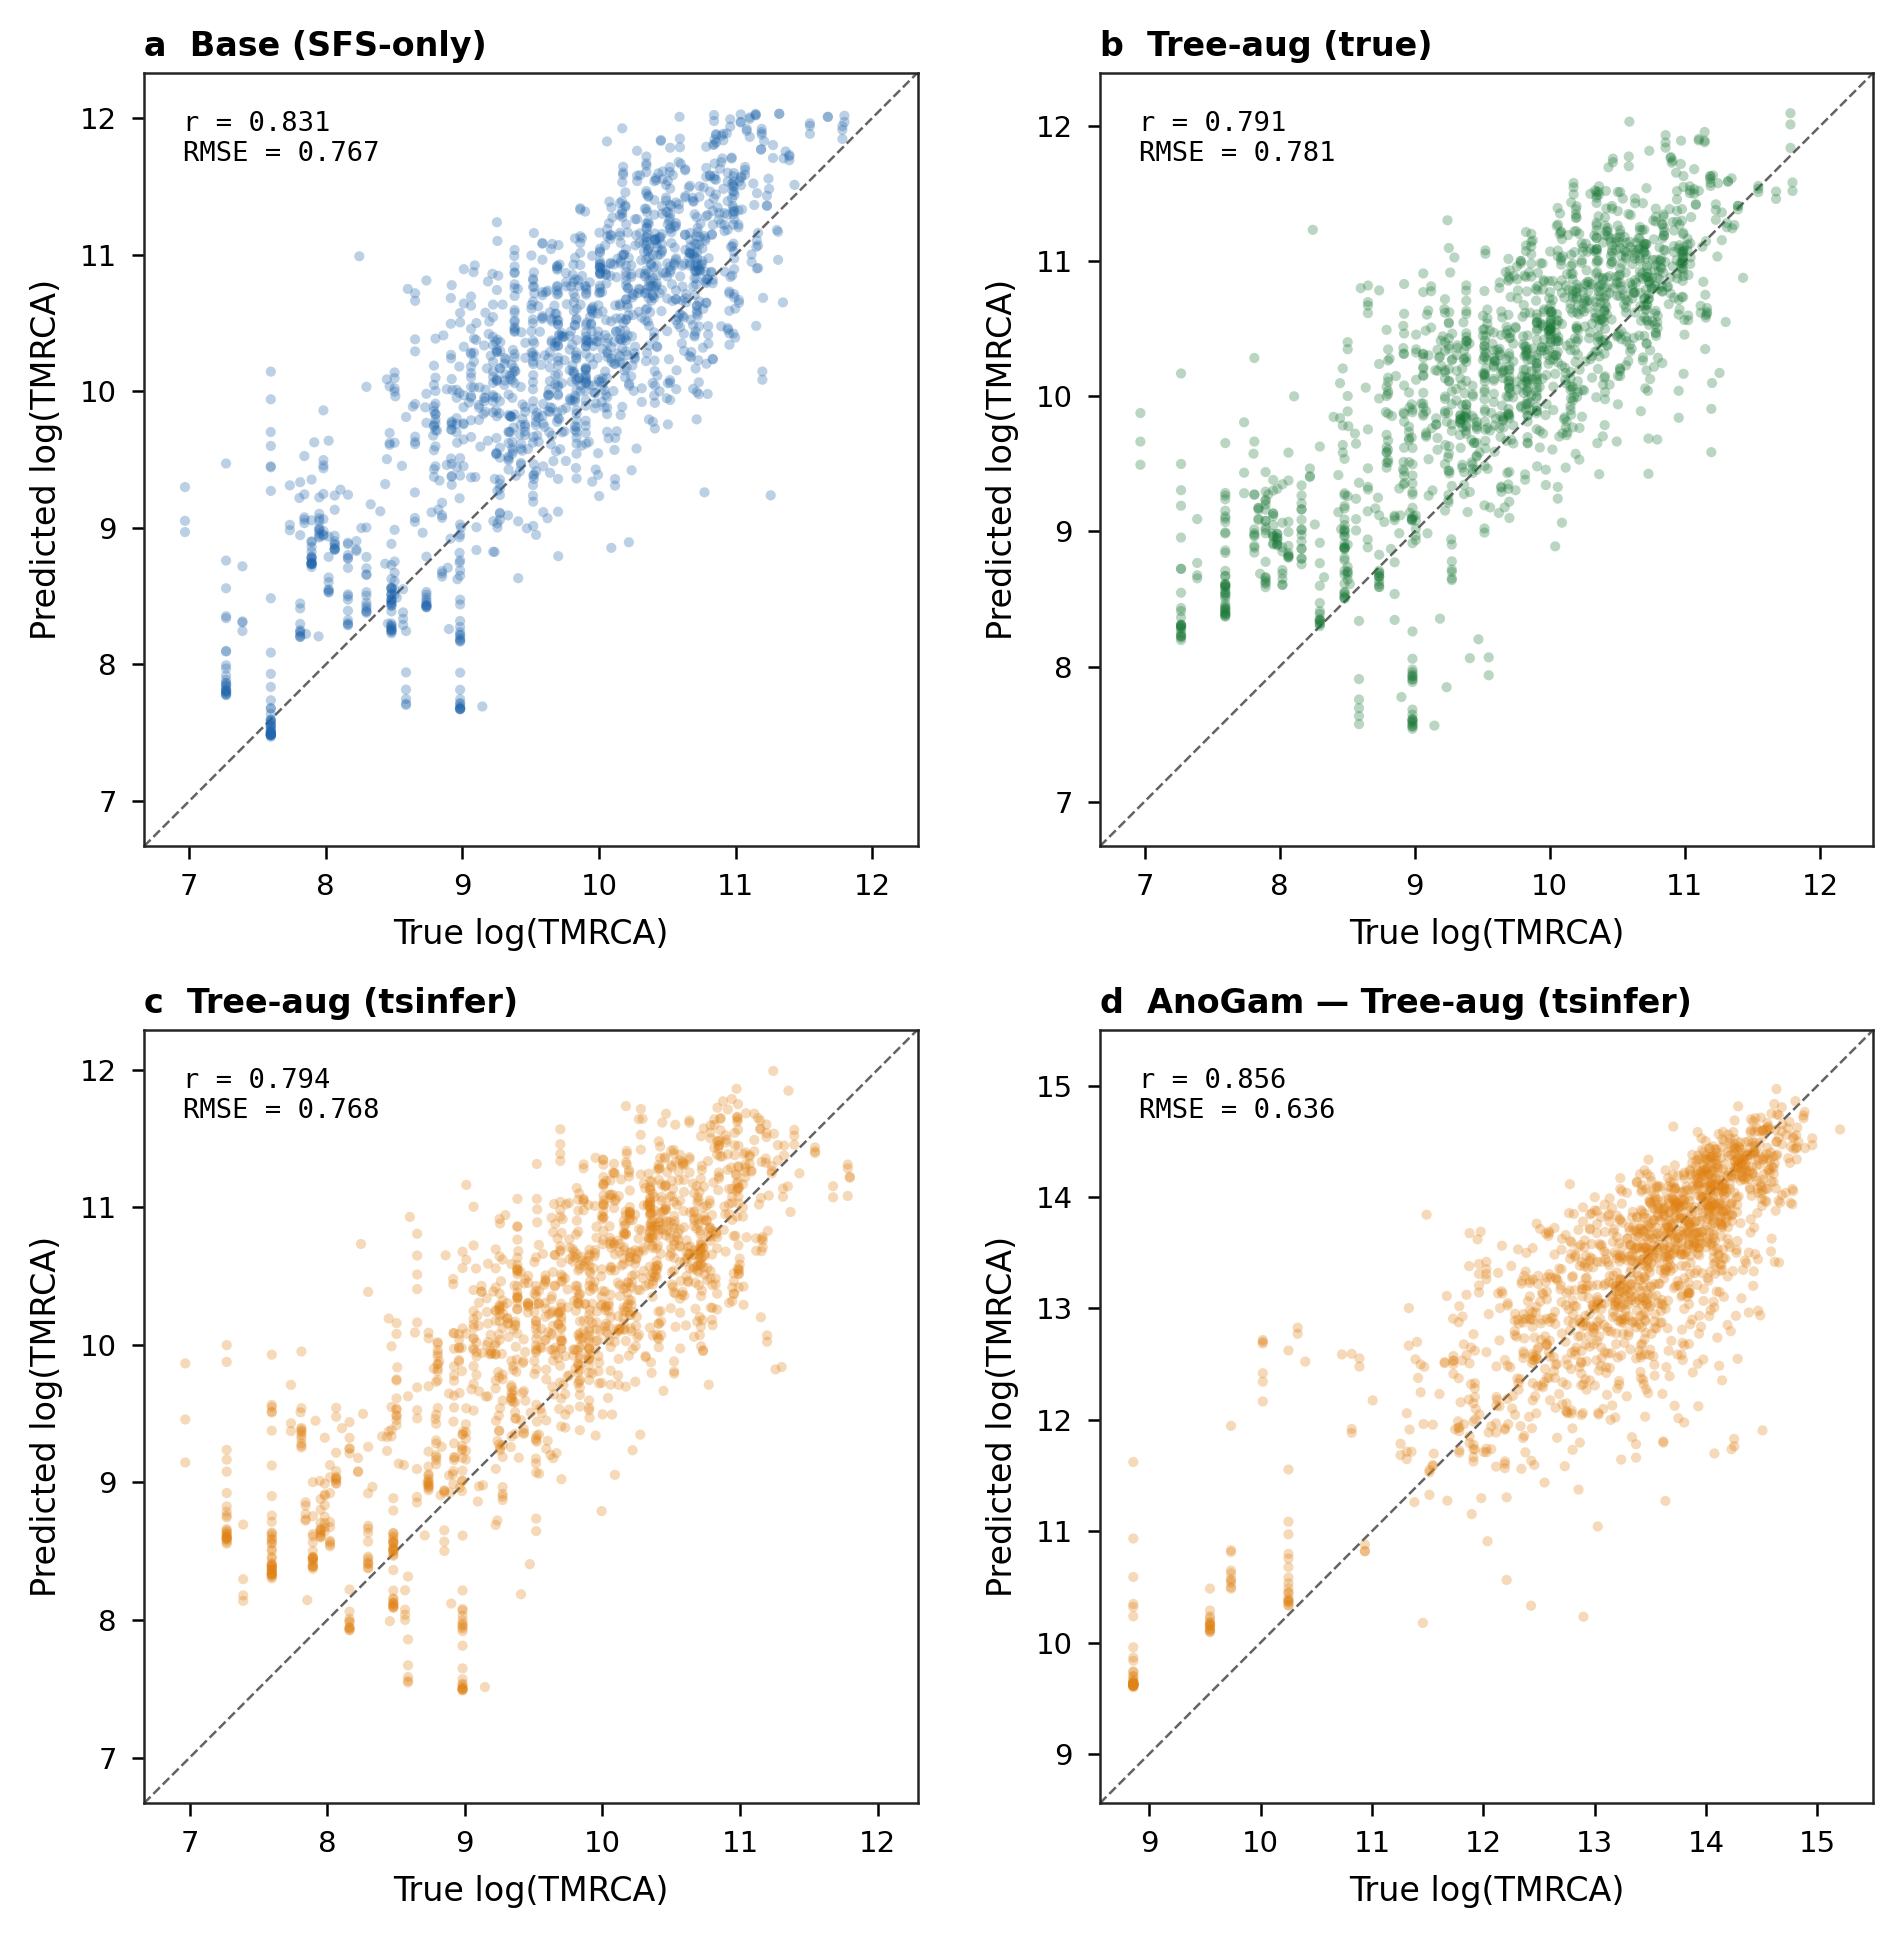
\includegraphics[width=\textwidth]{fig2_combined.png}\\[4pt]
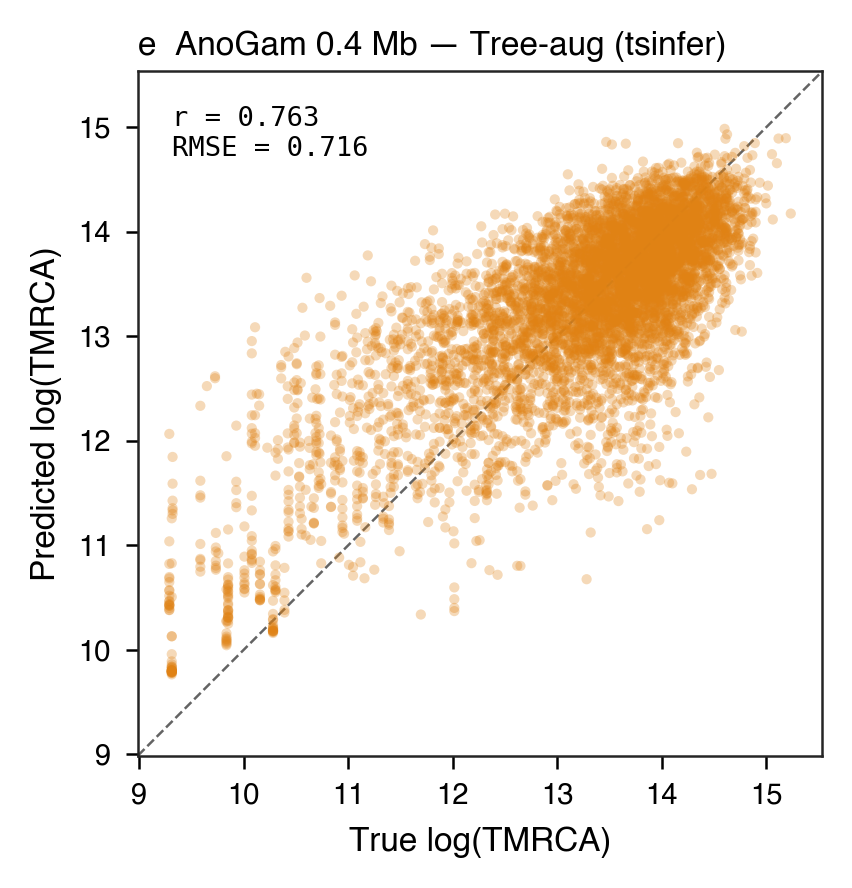
\includegraphics[width=0.42\textwidth]{fig2e_scatter_400kb.png}
\caption{True vs.\ predicted log(TMRCA). (a)~Base (SFS-only), (b)~tree-aug (true trees),
(c)~tree-aug (tsinfer)---all on human-like 1\,Mb simulations; (d)~tree-aug (tsinfer) on
\emph{Anopheles gambiae} (100\,kb, 500 windows); (e)~same architecture on AnoGam 400\,kb
with 2{,}000 windows. Dashed line: perfect prediction.}
\label{fig:scatter}
\end{figure}

\subsection{TMRCA Along the Genome}

Figure~\ref{fig:genome} shows predicted TMRCA profiles for one focal pair on 1\,Mb (top),
100\,kb AnoGam (middle), and 400\,kb AnoGam (bottom). All models capture peaks and valleys
in coalescence time, resolve rapid transitions at recombination breakpoints, and produce
well-calibrated $\pm 1$\,s.d.\ uncertainty bands.

\begin{figure}[t]
\centering
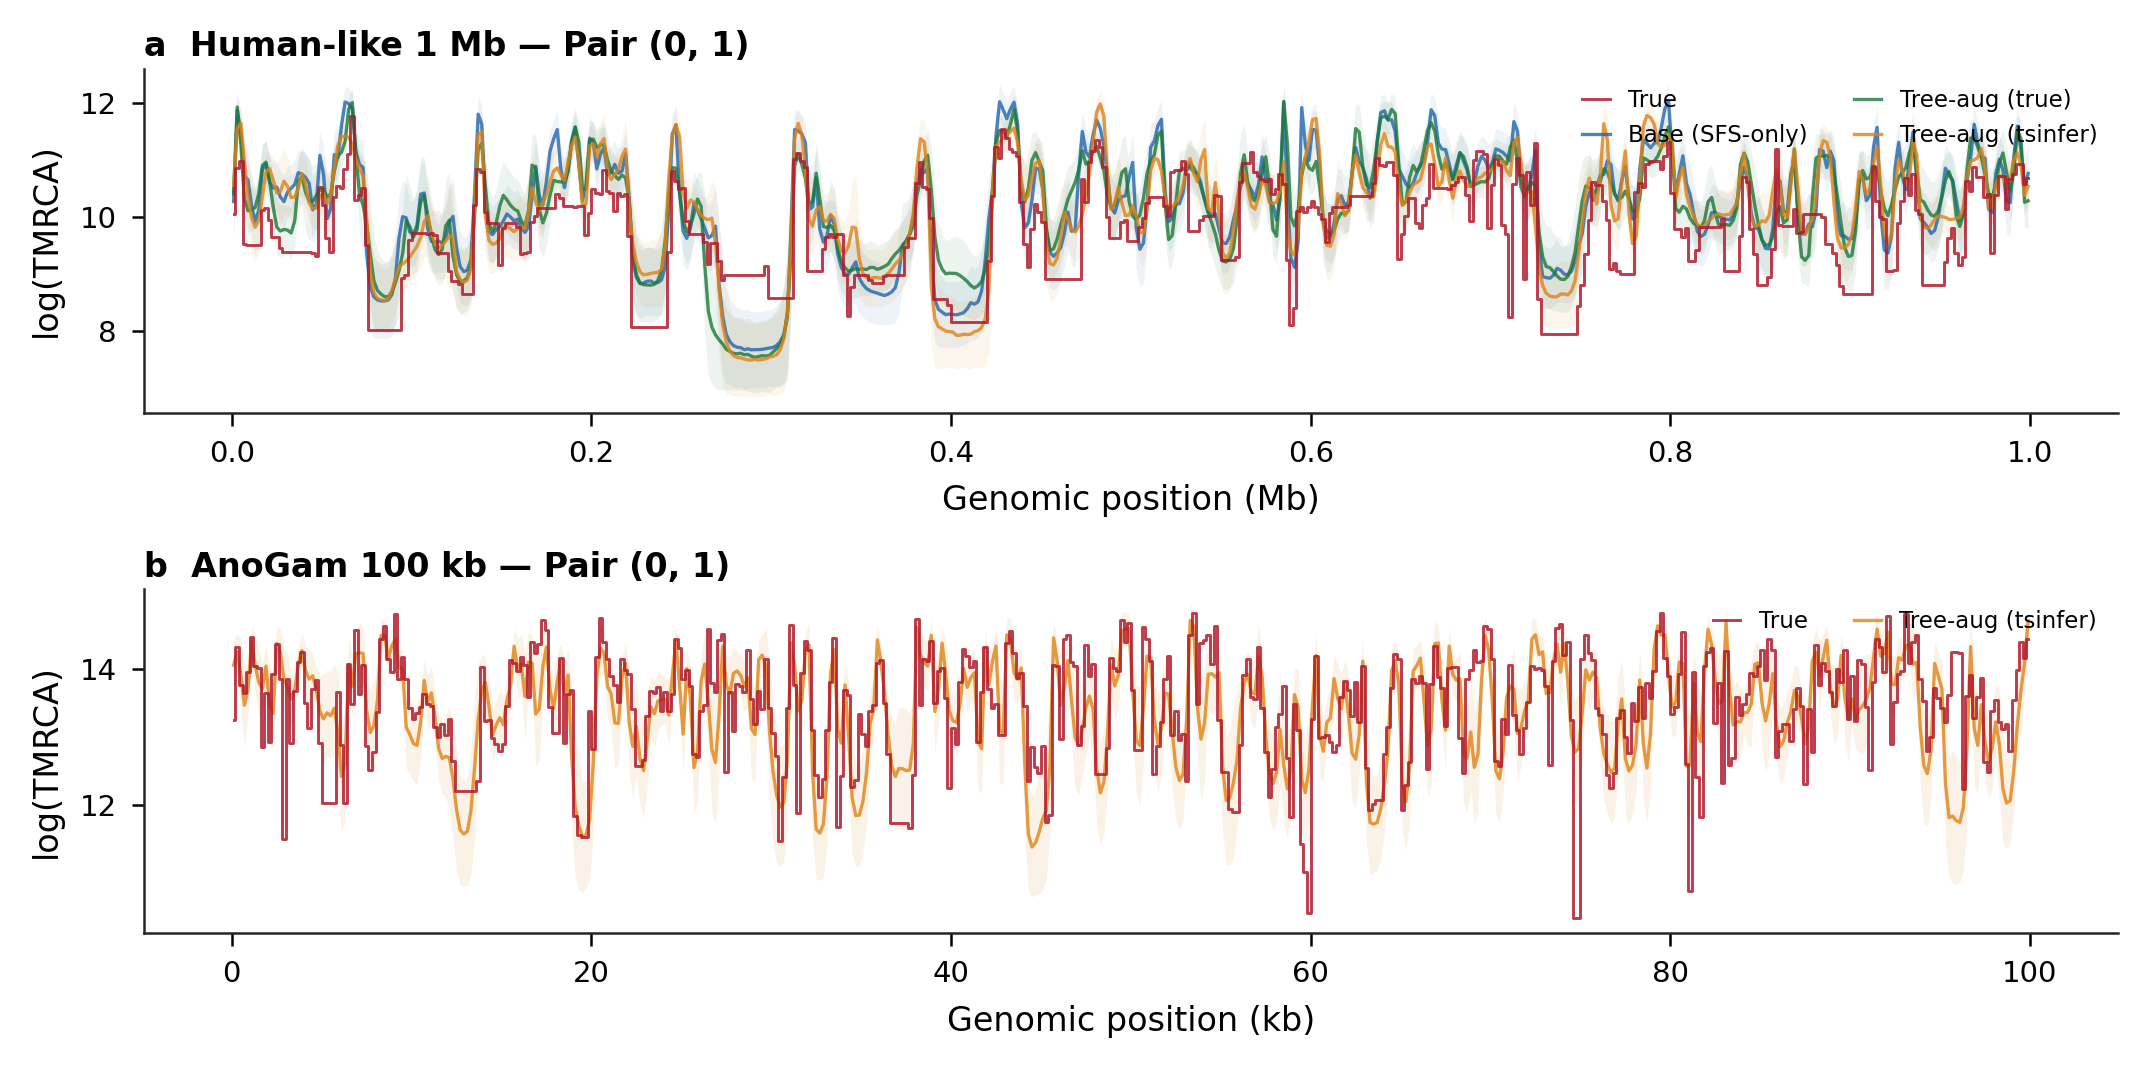
\includegraphics[width=\textwidth]{fig3_combined.png}\\[2pt]
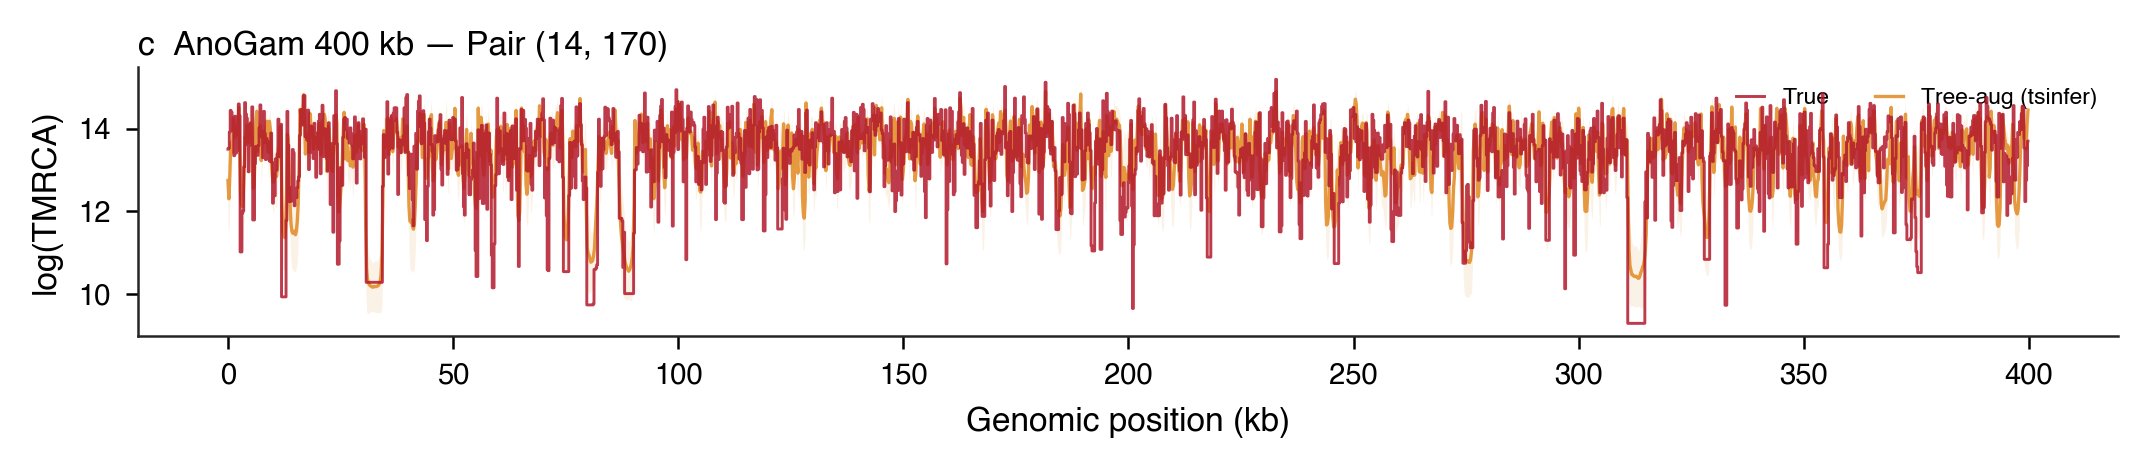
\includegraphics[width=\textwidth]{fig3c_genome_400kb.png}
\caption{Predicted TMRCA along the genome for a single focal pair.
(a)~Human-like 1\,Mb---red = true; blue = base; green = tree-aug (true); orange = tree-aug (tsinfer).
(b)~AnoGam 100\,kb---red = true; orange = tree-aug (tsinfer).
(c)~AnoGam 400\,kb (2{,}000 windows)---same color scheme. Shaded: $\pm 1$\,s.d.}
\label{fig:genome}
\end{figure}

\subsection{Cross-Species Transfer: \emph{Anopheles gambiae}}
\label{sec:anogam}

To test whether the architecture generalizes beyond the constant-size human-like
demographic model, we train a tree-augmented (tsinfer) model on
\emph{Anopheles gambiae} (AnoGam) data simulated with
\texttt{stdpopsim}~\citep{adrion2020community}: 100\,kb segments, 200\,bp windows
(500 windows), same sample sizes and hyperparameters as above. Panel~(d) of
Figure~\ref{fig:scatter} and panel~(b) of Figure~\ref{fig:genome} show scatter
and genome profiles; Table~\ref{tab:accuracy} reports $r = 0.804$, RMSE\;$0.646$.
The \textsc{fastcxt} architecture thus transfers to a non-human species without
architectural changes.

\paragraph{Scaling to longer context (400\,kb, 2{,}000 windows).}
To explore whether the same architecture can handle $4\times$ longer genomic context,
we train an identical model ($d_\mathrm{model} = 256$, 17.2M parameters) on 400\,kb
AnoGam segments tiled into 2{,}000 windows of 200\,bp each. Because Mamba processes
sequences in $O(L)$ time, the only change is the sequence length $W$; no architectural
modifications are needed. On three held-out test pairs the model achieves
$r = 0.763$, RMSE\;$0.716$ (panel~e of Figure~\ref{fig:scatter}, panel~c of
Figure~\ref{fig:genome}). While accuracy is lower than the 100\,kb variant---expected
given that longer segments contain more recombination breakpoints and coalescent
variation---the result demonstrates that Mamba's linear scaling enables practical
inference over substantially longer contexts, with wall time growing approximately
linearly (${\sim}4\times$) rather than quadratically as attention-based architectures
would require.

% \subsection{Out-of-Distribution Robustness}
%
% Figure~\ref{fig:ood} evaluates model robustness under misspecified demographic parameters.
% We vary $N_e$ and $\mu$ jointly over a $2\times$ log-spaced grid around the training values
% and measure prediction bias and MSE. The base model remains well-calibrated near the training
% regime and degrades gracefully: bias is approximately zero within a 2-fold parameter range,
% and MSE increases smoothly without catastrophic failure, confirming that the learned
% representation captures genuine coalescent structure rather than overfitting to a narrow
% parameter point.
%
% \begin{figure}[t]
% \centering
% 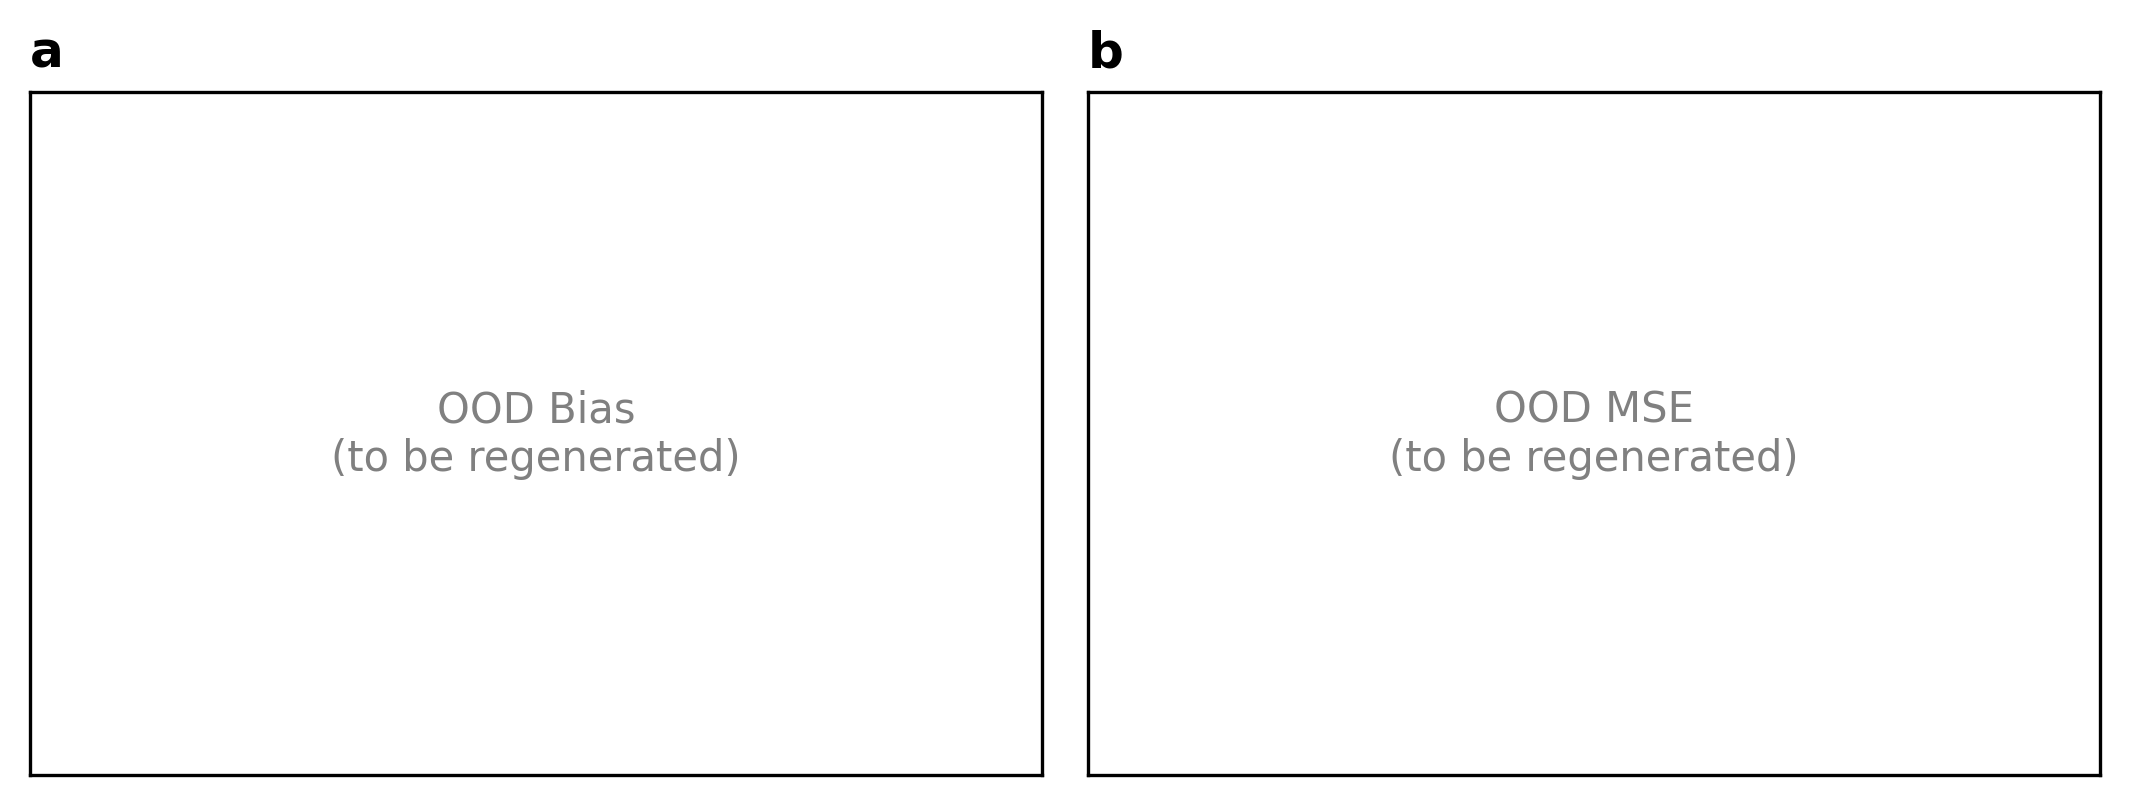
\includegraphics[width=\textwidth]{fig4_ood.png}
% \caption{Out-of-distribution robustness. (a)~Prediction bias and (b)~MSE as $N_e$ and $\mu$
% are scaled relative to training values (green dot). The model degrades gracefully under
% demographic misspecification.}
% \label{fig:ood}
% \end{figure}

\subsection{Computational Scaling}

\begin{table}[t]
\caption{Benchmark: inference time (seconds) for all pairwise TMRCAs at varying sample sizes.
``Node-time'': Mamba forward pass + LCA lookups; ``Full pipeline'': tsinfer + node-time.
Speedup columns show the ratio of pairwise time to node-time (NT) or full-pipeline (Full) time.}
\label{tab:benchmark}
\centering
\small
\begin{tabular}{rrcccccc}
\toprule
$n$ & Pairs & Pairwise & Node-time & tsinfer & Full & \multicolumn{2}{c}{Speedup} \\
\cmidrule(lr){7-8}
    &       & (s) & (s) & (s) & (s) & NT & Full \\
\midrule
 30 &   435 &  1.80 & 0.25 & 0.70 & 0.96 &  7$\times$ & 2$\times$ \\
 50 & 1{,}225 &  5.52 & 0.71 & 1.02 & 1.72 &  8$\times$ & 3$\times$ \\
 75 & 2{,}775 & 14.47 & 1.60 & 1.41 & 3.01 &  9$\times$ & 5$\times$ \\
100 & 4{,}950 & 33.36 & 2.94 & 1.86 & 4.80 & 11$\times$ & 7$\times$ \\
\bottomrule
\end{tabular}
\end{table}

Table~\ref{tab:benchmark} and Figure~\ref{fig:scaling} show scaling results. The pairwise model
follows the expected $O(n^2)$ curve, reaching 33.4\,s for $n = 100$. The node-time model alone
scales approximately linearly, completing the same task in 2.9\,s---an $11\times$ speedup.
Including tsinfer in the full pipeline, inference at $n = 100$ takes ${\sim}4.8$\,s, a
$7\times$ speedup over pairwise. Extrapolating, the pairwise model would require ${>}3$\,h
for $n = 1{,}000$ haplotypes while the full pipeline remains in the seconds.

\paragraph{Sequence-length scaling.}
Independently of sample-size scaling, Mamba's $O(L)$ complexity in sequence length enables
processing longer genomic context without architectural changes. The 400\,kb AnoGam model uses
the same architecture ($d_\mathrm{model} = 256$, 17.2M parameters) as the 100\,kb variant but
processes $W = 2{,}000$ windows instead of 500. Wall time per forward pass increases approximately
$4\times$---linearly with context length---whereas an attention-based architecture would incur
$16\times$ cost. A detailed wall-time-per-bp benchmark across context lengths is deferred to
future work.

\begin{figure}[t]
\centering
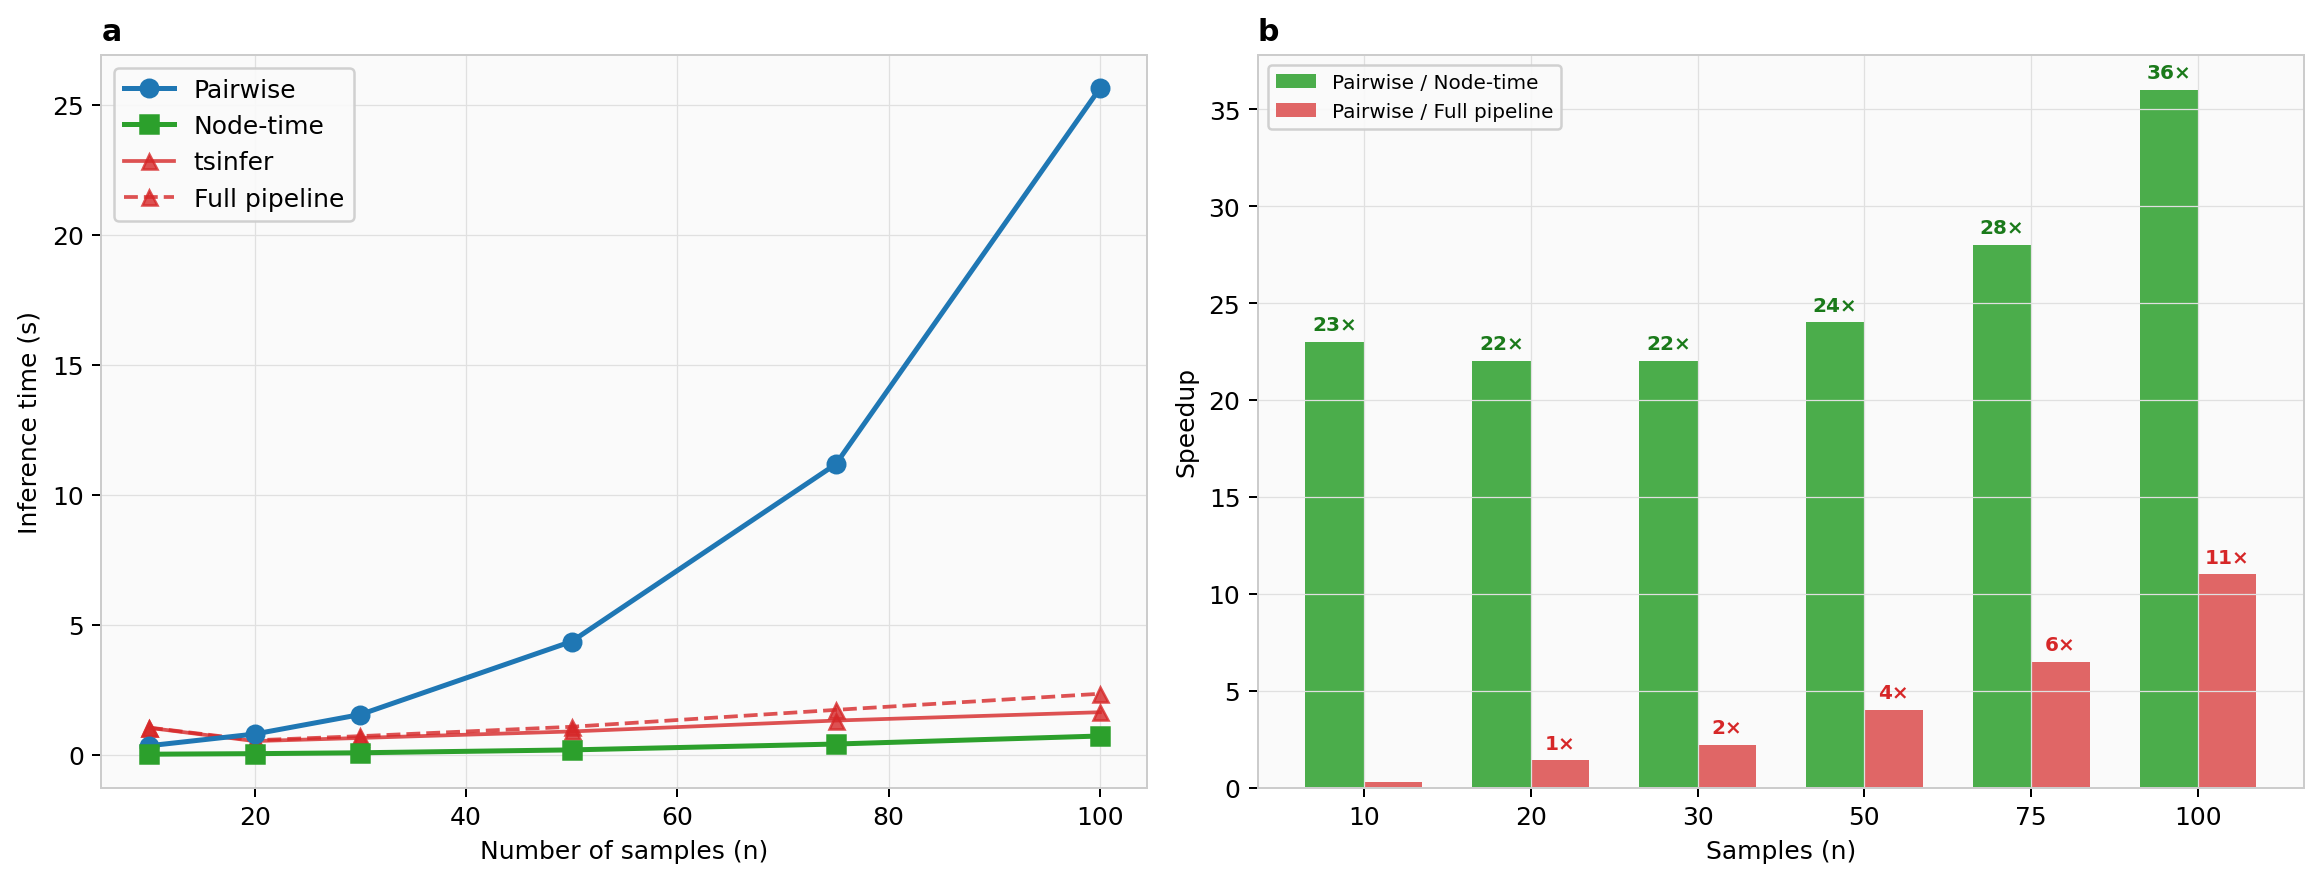
\includegraphics[width=\textwidth]{fig5_scaling.png}
\caption{Computational scaling (human-like 1\,Mb setup). (a)~Inference time vs.\ sample size.
(b)~Speedup over the pairwise model: node-time only (NT) and full pipeline including tsinfer (Full).
The same scaling applies to the AnoGam (100\,kb) pipeline.}
\label{fig:scaling}
\end{figure}

\subsection{Real Data Application: Ag1000G Chromosome 2L}
\label{sec:ag1000g}

To demonstrate \textsc{fastcxt} on real data, we apply the AnoGam-trained model to
chromosome~2L of the Ag1000G phase~3 release~\citep{ag1000g2021}, which provides
a \texttt{tsinfer}-inferred and \texttt{tsdate}-dated tree sequence for 1{,}470
\emph{Anopheles gambiae} individuals across 16 African populations.
We focus on the 25 Burkina Faso individuals heterozygous for the 2La chromosomal
inversion (\texttt{2La\,=\,1}), yielding 50 haploid samples and 190 focal pairs
(25 within-individual plus 165 between-individual).

\paragraph{Missing data handling.}
The Ag1000G accessibility mask flags ${\sim}27\%$ of 2L sites as inaccessible due to
low mappability or repetitive content. Before building the SFS input, we filter out
all variant sites at inaccessible positions. The model receives no explicit
missingness signal---it simply observes sparser SFS vectors in windows with fewer
accessible bases. In principle, windows with many masked sites could appear
artificially depleted of mutations, biasing TMRCA estimates upward. In practice,
the per-pair diversity-based bias correction (described below) compensates for this
at the genome-wide level, and the model's heteroscedastic output assigns wider
uncertainty to data-poor windows. The tree topology features, extracted from the
full (unmasked) genealogy, further anchor predictions in regions where the SFS is
sparse.

\paragraph{Inference protocol.}
After simplifying the tree sequence to the 50 focal haploids (1.83M sites, 1.74M
accessible), we tile chromosome~2L into 493 non-overlapping 100\,kb blocks
(200\,bp windows, 500 per block). Since the Ag1000G release already provides a
\texttt{tsinfer}-inferred tree sequence, we extract topology features directly
from the existing genealogy for each block and pair them with the SFS input,
running the trained tree-augmented pairwise model with the \emph{Anopheles}
mutation rate $\mu = 3.5 \times 10^{-9}$/bp/generation. Following
\texttt{cxt}~\citep{korfmann2025cxt}, we apply a per-pair diversity-based bias
correction that aligns the predicted genome-wide mean diversity
$2\mu\overline{\exp(\hat{y})}$ with the observed pairwise diversity from the tree
sequence, yielding a small additive shift in log-space (${\sim}0.06$).

\paragraph{Results.}
Figure~\ref{fig:ag1000g} shows the inferred coalescence-time landscape.
Panel~(a) displays a density heatmap of predicted log(TMRCA) for within-individual
pairs across the 49.4\,Mb arm (position $\times$ coalescence depth, colored by
density). Two salient features emerge: (i)~a pronounced upward shift in
coalescence depth at the 2La inversion breakpoints (${\sim}$20.5 and
${\sim}$42.2\,Mb), consistent with suppressed recombination within the inversion
maintaining deeply divergent haplotype blocks in heterozygotes; and
(ii)~localized dips in coalescence time, notably around the Rdl
insecticide-resistance locus (${\sim}$25.4\,Mb), indicative of a recent selective
sweep.
Panel~(b) overlays the \textsc{fastcxt} population-mean log(TMRCA) (block-level
averages across within-individual pairs) with the corresponding \texttt{tsdate}
estimates from the Ag1000G dated tree sequence, rescaled to the same mutation rate
($\mu_\text{tsdate} = 10^{-9}$; $\mu_\text{AnoGam} = 3.5 \times 10^{-9}$).
The two methods track each other closely across the chromosome, both resolving
the 2La inversion step and the Rdl sweep dip, validating \textsc{fastcxt} against
an independent dating method on real data.

\begin{figure}[t]
\centering
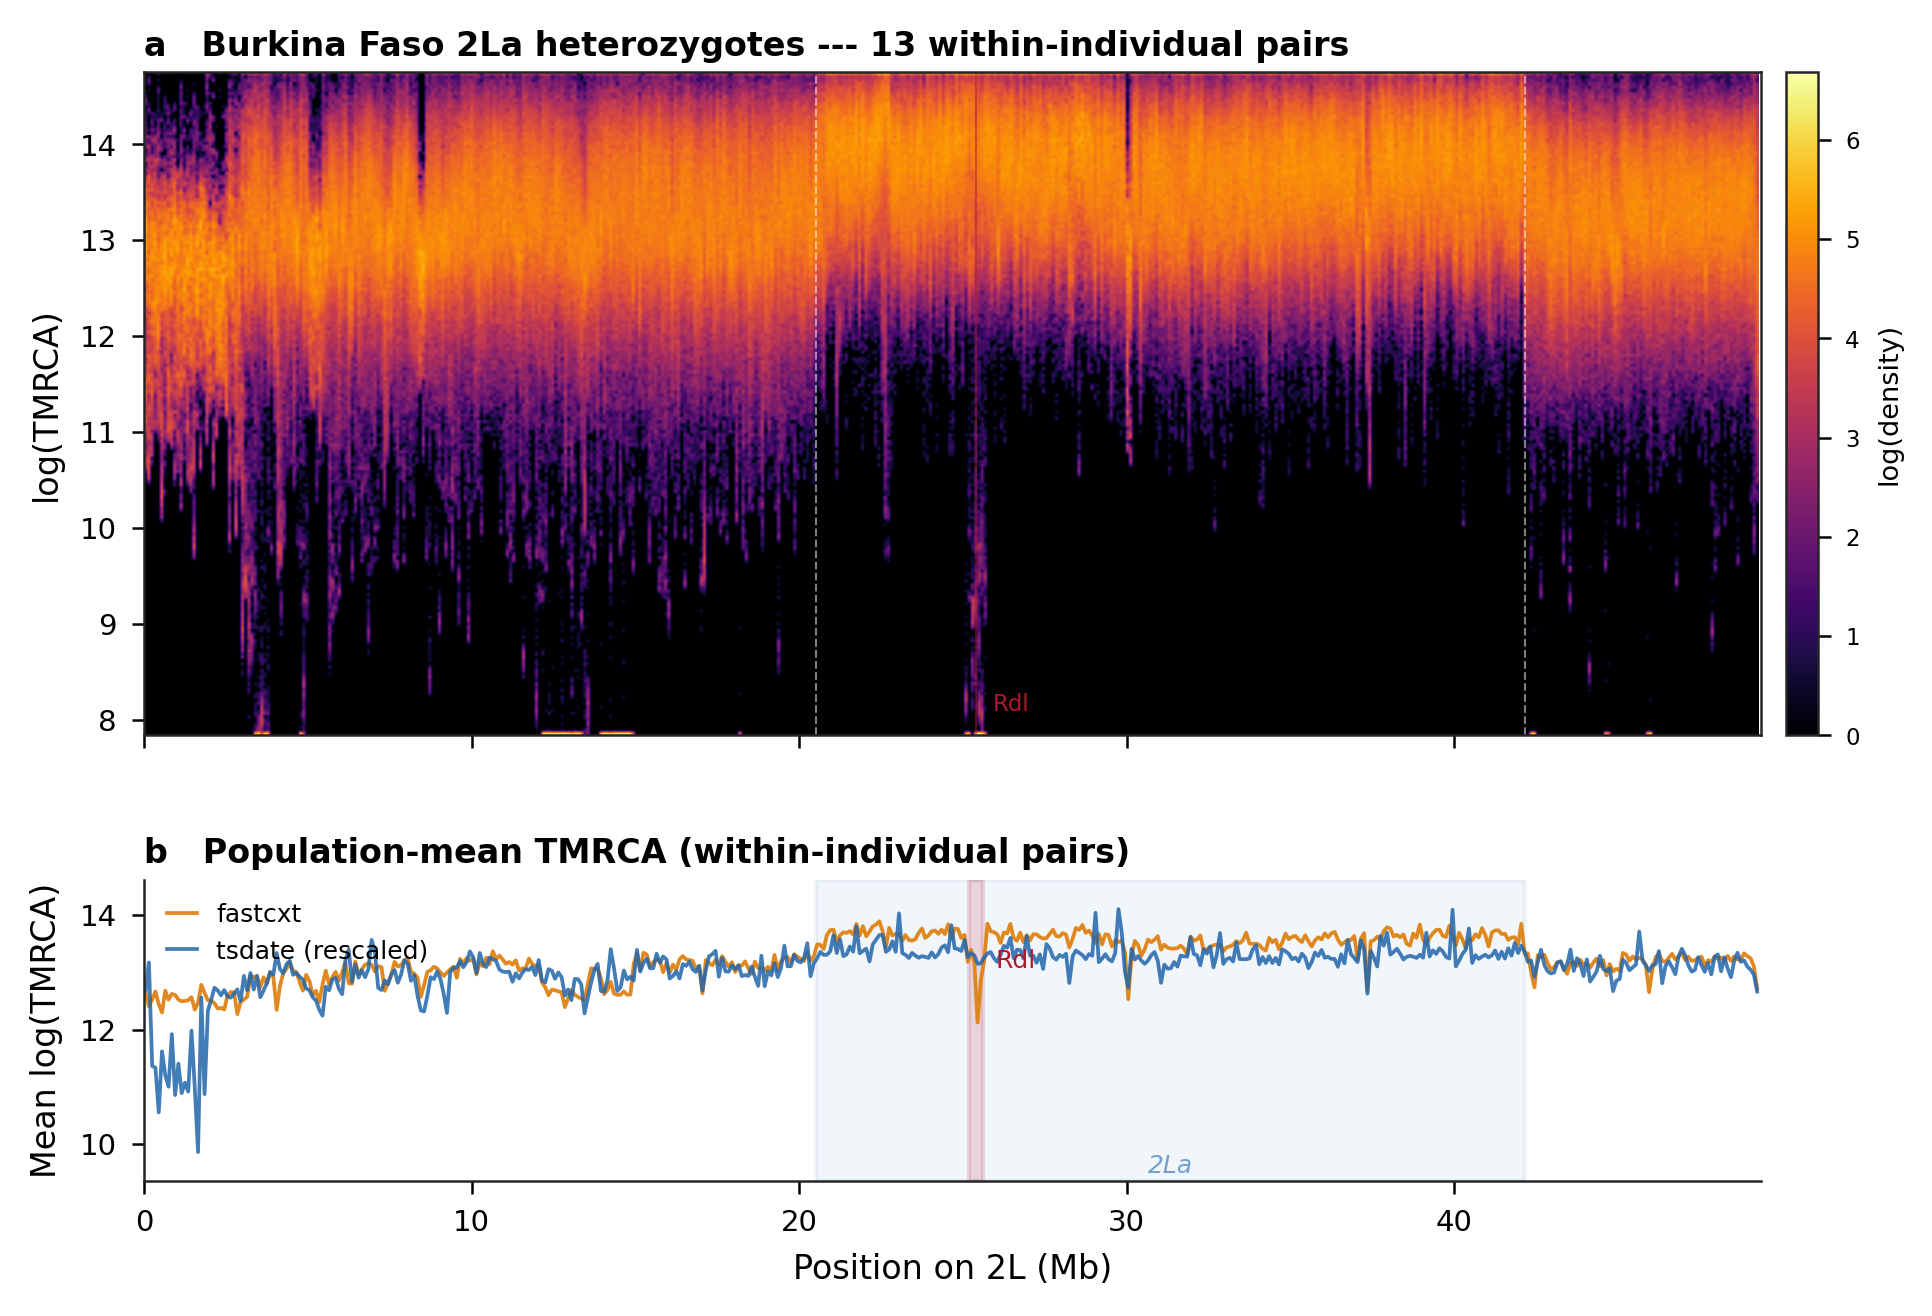
\includegraphics[width=\textwidth]{fig_ag1000g_2L.png}
\caption{Pairwise coalescence times across \emph{An.\,gambiae} chromosome~2L
(Ag1000G, Burkina Faso 2La heterozygotes).
(a)~Density heatmap: position $\times$ log(TMRCA) for within-individual pairs;
dashed lines mark 2La inversion breakpoints.
(b)~Population-mean log(TMRCA) for \textsc{fastcxt} (orange) and \texttt{tsdate}
(blue, rescaled to $\mu = 3.5 \times 10^{-9}$); blue shading marks the 2La
inversion, red marks the Rdl locus.}
\label{fig:ag1000g}
\end{figure}

\section{Discussion}

\paragraph{From cxt to fastcxt.}
\texttt{cxt}~\citep{korfmann2025cxt} demonstrated that TMRCA inference can be cast as a
language-modeling task, autoregressively predicting coalescence events from mutation patterns.
\textsc{fastcxt} retains the same SFS-based input representation and the core insight that
local mutation context is informative about the latent genealogy, but replaces the
autoregressive transformer with a non-autoregressive bidirectional Mamba encoder--decoder.
This eliminates the sequential decode bottleneck: the 6-layer encoder processes 500-window
sequences in ${\sim}200$\,ms on a single GPU. The node-time model further removes the
$O(n^2)$ pair enumeration, providing 7--11$\times$ speedup over the pairwise Mamba baseline.
In practice, \textsc{fastcxt} completes genome-wide inference in seconds where \texttt{cxt}
requires minutes, making whole-genome analysis feasible by tiling the chromosome into
overlapping 1\,Mb blocks.

\paragraph{Tree topology features.}
Topology features carry complementary information to the SFS. The SFS captures marginal
mutation patterns but is inherently lossy---many tree shapes produce the same SFS. The tree
features disambiguate these degeneracies by directly encoding coalescent rank order, subtree
sizes, and split balance. The tsinfer-augmented model achieves the best performance
($r = 0.887$), demonstrating that even imperfectly inferred trees provide useful signal, while
the base model's competitive accuracy ($r = 0.879$) makes it a strong standalone method when
tree inference is unavailable.

\paragraph{Breaking the $O(n^2)$ barrier.}
The node-time model shifts from pair-centric to tree-centric inference, predicting all internal
node times simultaneously; pairwise TMRCAs are recovered via LCA lookups. This factored design
also enables richer downstream queries---$k$-sample MRCAs, clade-level divergence summaries,
or time-stratified genealogical statistics---without rerunning the neural network.

\paragraph{Calibrated uncertainty.}
The heteroscedastic Gaussian output trained with Beta-NLL loss provides calibrated uncertainty
(Figure~\ref{fig:residuals}): approximately centered, symmetric residuals with no spatial bias.

\paragraph{Cross-species generalization and longer context.}
The AnoGam experiments (Section~\ref{sec:anogam}) show that \textsc{fastcxt}'s architecture transfers
without modification to a non-human species with different effective population size,
recombination landscape, and demographic history---requiring only species-appropriate
simulation data and adjusted window size. The 400\,kb variant ($W = 2{,}000$) further
demonstrates that the same 17.2M-parameter model scales to $4\times$ longer genomic
context with approximately linear wall-time increase, a direct benefit of Mamba's
$O(L)$ complexity.

\paragraph{Real data validation.}
The Ag1000G application (Section~\ref{sec:ag1000g}) demonstrates that \textsc{fastcxt}
recovers biologically meaningful coalescence-time variation on real data. The 2La inversion
boundaries and the Rdl selective-sweep signal are clearly resolved, and predicted
TMRCA profiles closely match independent \texttt{tsdate} estimates after accounting for
the mutation-rate difference between the Ag1000G dating pipeline ($\mu = 10^{-9}$) and
the \texttt{stdpopsim} AnoGam rate ($\mu = 3.5 \times 10^{-9}$). The per-pair
diversity-based bias correction from \texttt{cxt}~\citep{korfmann2025cxt} provides a
principled post-hoc calibration, aligning predicted and observed diversity with a small
log-space shift.

\paragraph{Limitations.}
The AnoGam model was trained on the \texttt{GabonAg1000G\_1A17} demographic model from
\texttt{stdpopsim}, which approximates the coalescent-depth distribution of a single
Gabonese population. Application to other populations (e.g., Burkina Faso) introduces
a demographic mismatch that the diversity correction partially addresses. Training on
a broader set of demographic scenarios---or directly on population-matched
models---would further improve absolute calibration. Hierarchical block-boundary handling
and explicit modeling of natural selection remain important directions.

\section{Related Work}

\paragraph{Coalescence time inference.}
PSMC~\citep{li2011inference} and MSMC~\citep{schiffels2014inferring} pioneered HMM-based TMRCA
inference; tree-sequence methods (Relate~\citep{speidel2019method},
tsinfer~\citep{kelleher2019inferring}, tsdate~\citep{wohns2022unified}) infer full genealogies.
Gamma-SMC~\citep{schweiger2023ultrafast} provides ultrafast pairwise inference but retains
$O(n^2)$ scaling. \texttt{cxt}~\citep{korfmann2025cxt} introduced the language-modeling
paradigm for coalescent inference; \textsc{fastcxt} builds on it with non-autoregressive
Mamba processing, tree augmentation, and the node-time formulation for linear scaling.

\paragraph{Deep learning in population genetics.}
Neural networks have been applied to demographic inference~\citep{flagel2019unreasonable},
selection detection~\citep{kern2018diploShic}, and recombination-rate
estimation~\citep{adrion2020community}. Mamba has been used for DNA sequence
modeling~\citep{schiff2024caduceus}; our application processes a derived representation
(windowed SFS) at kilobase resolution.

\section{Conclusion}

Building on the language-modeling paradigm introduced by \texttt{cxt}~\citep{korfmann2025cxt},
\textsc{fastcxt} replaces the autoregressive transformer with a non-autoregressive
bidirectional Mamba encoder--decoder and introduces a node-time model that breaks the $O(n^2)$
scaling barrier of all pairwise methods, achieving $11\times$ speedup at $n=100$ with the
advantage growing as $O(n)$. Tree-augmented variants with tsinfer-inferred trees reach
$r = 0.887$, establishing end-to-end viability without access to the true genealogy.
On real \emph{Anopheles gambiae} data from the Ag1000G consortium, \textsc{fastcxt}
recovers the 2La inversion and Rdl selective-sweep signatures across chromosome~2L,
with predictions validated against independent \texttt{tsdate} estimates. Following
\texttt{cxt}'s demonstration of broad generalization across the \texttt{stdpopsim} catalog,
training \textsc{fastcxt} on diverse demographic scenarios is a natural next step toward
making genome-wide TMRCA inference practical at biobank scale.

\bibliographystyle{plainnat}
\bibliography{references}

\newpage
\appendix
\section{Supplementary Material}

\subsection{Training Dynamics}

\begin{figure}[h]
\centering
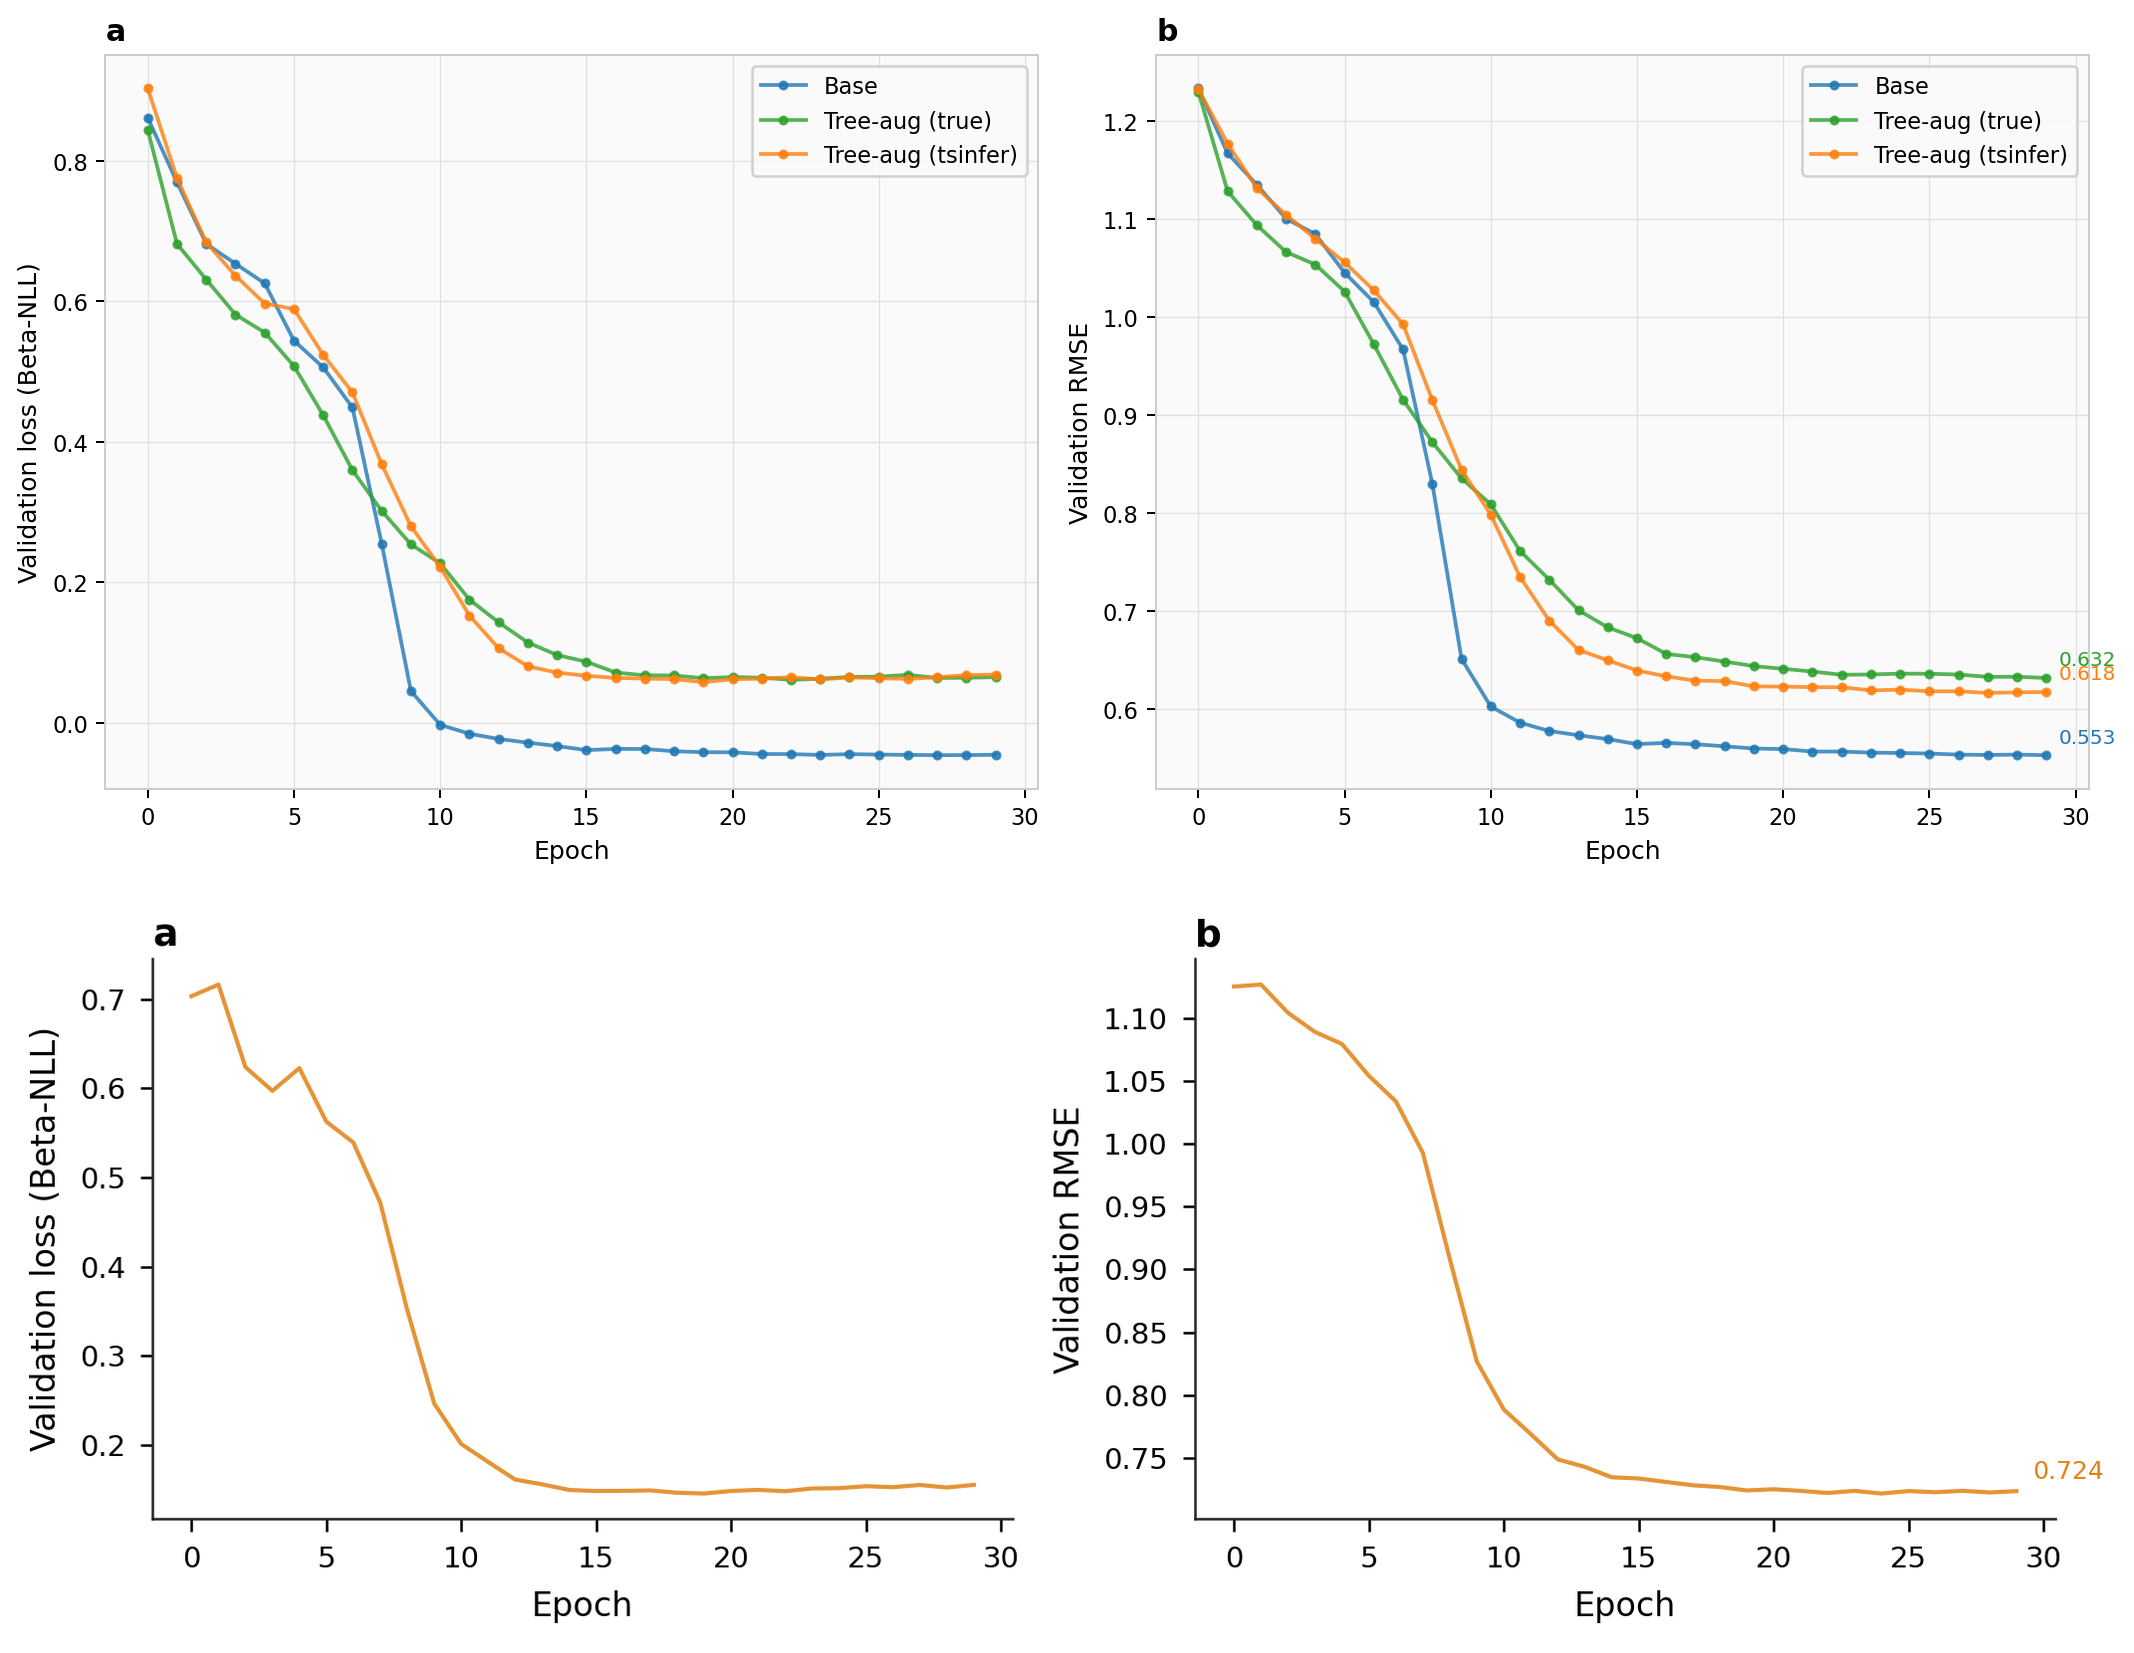
\includegraphics[width=\textwidth]{figS1_combined.png}\\[4pt]
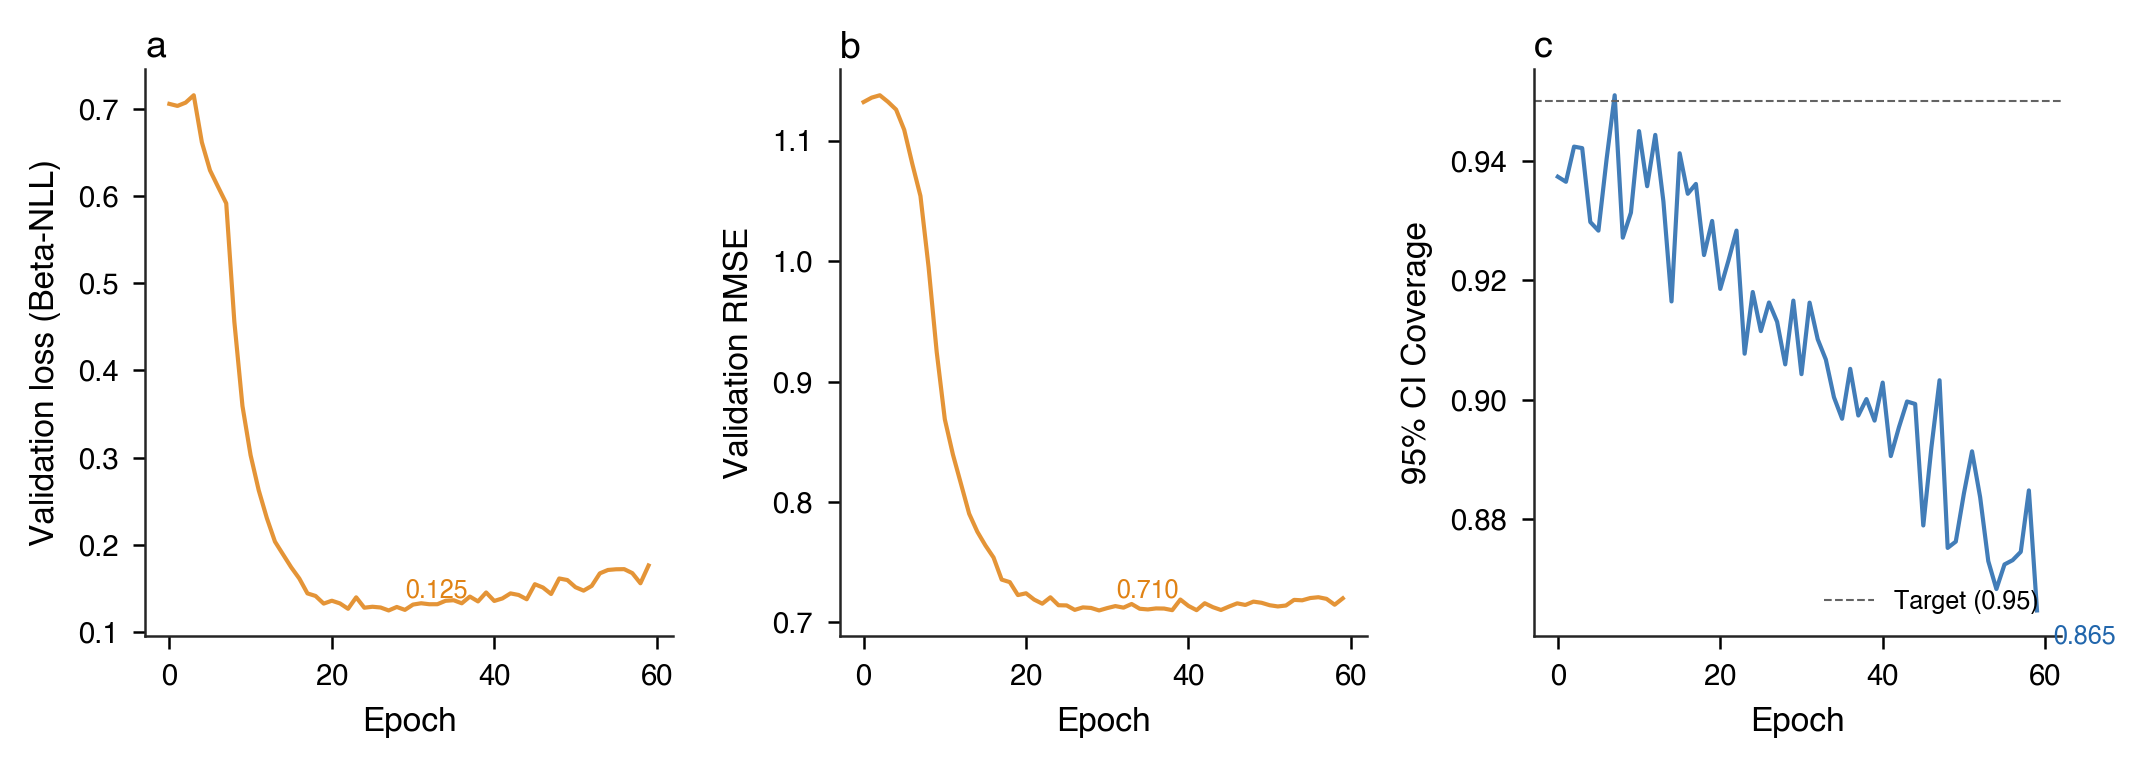
\includegraphics[width=0.48\textwidth]{training_2k.png}
\caption{Training dynamics (validation loss) over 30 epochs. (a)~Human-like models---blue:
base (SFS-only); green: tree-augmented (true trees); orange: tree-augmented (tsinfer).
(b)~AnoGam tree-augmented (tsinfer, 100\,kb). (c)~AnoGam tree-augmented (tsinfer, 400\,kb,
2{,}000 windows). All models converge smoothly without overfitting.}
\label{fig:training}
\end{figure}

\subsection{Residual Analysis}

\begin{figure}[h]
\centering
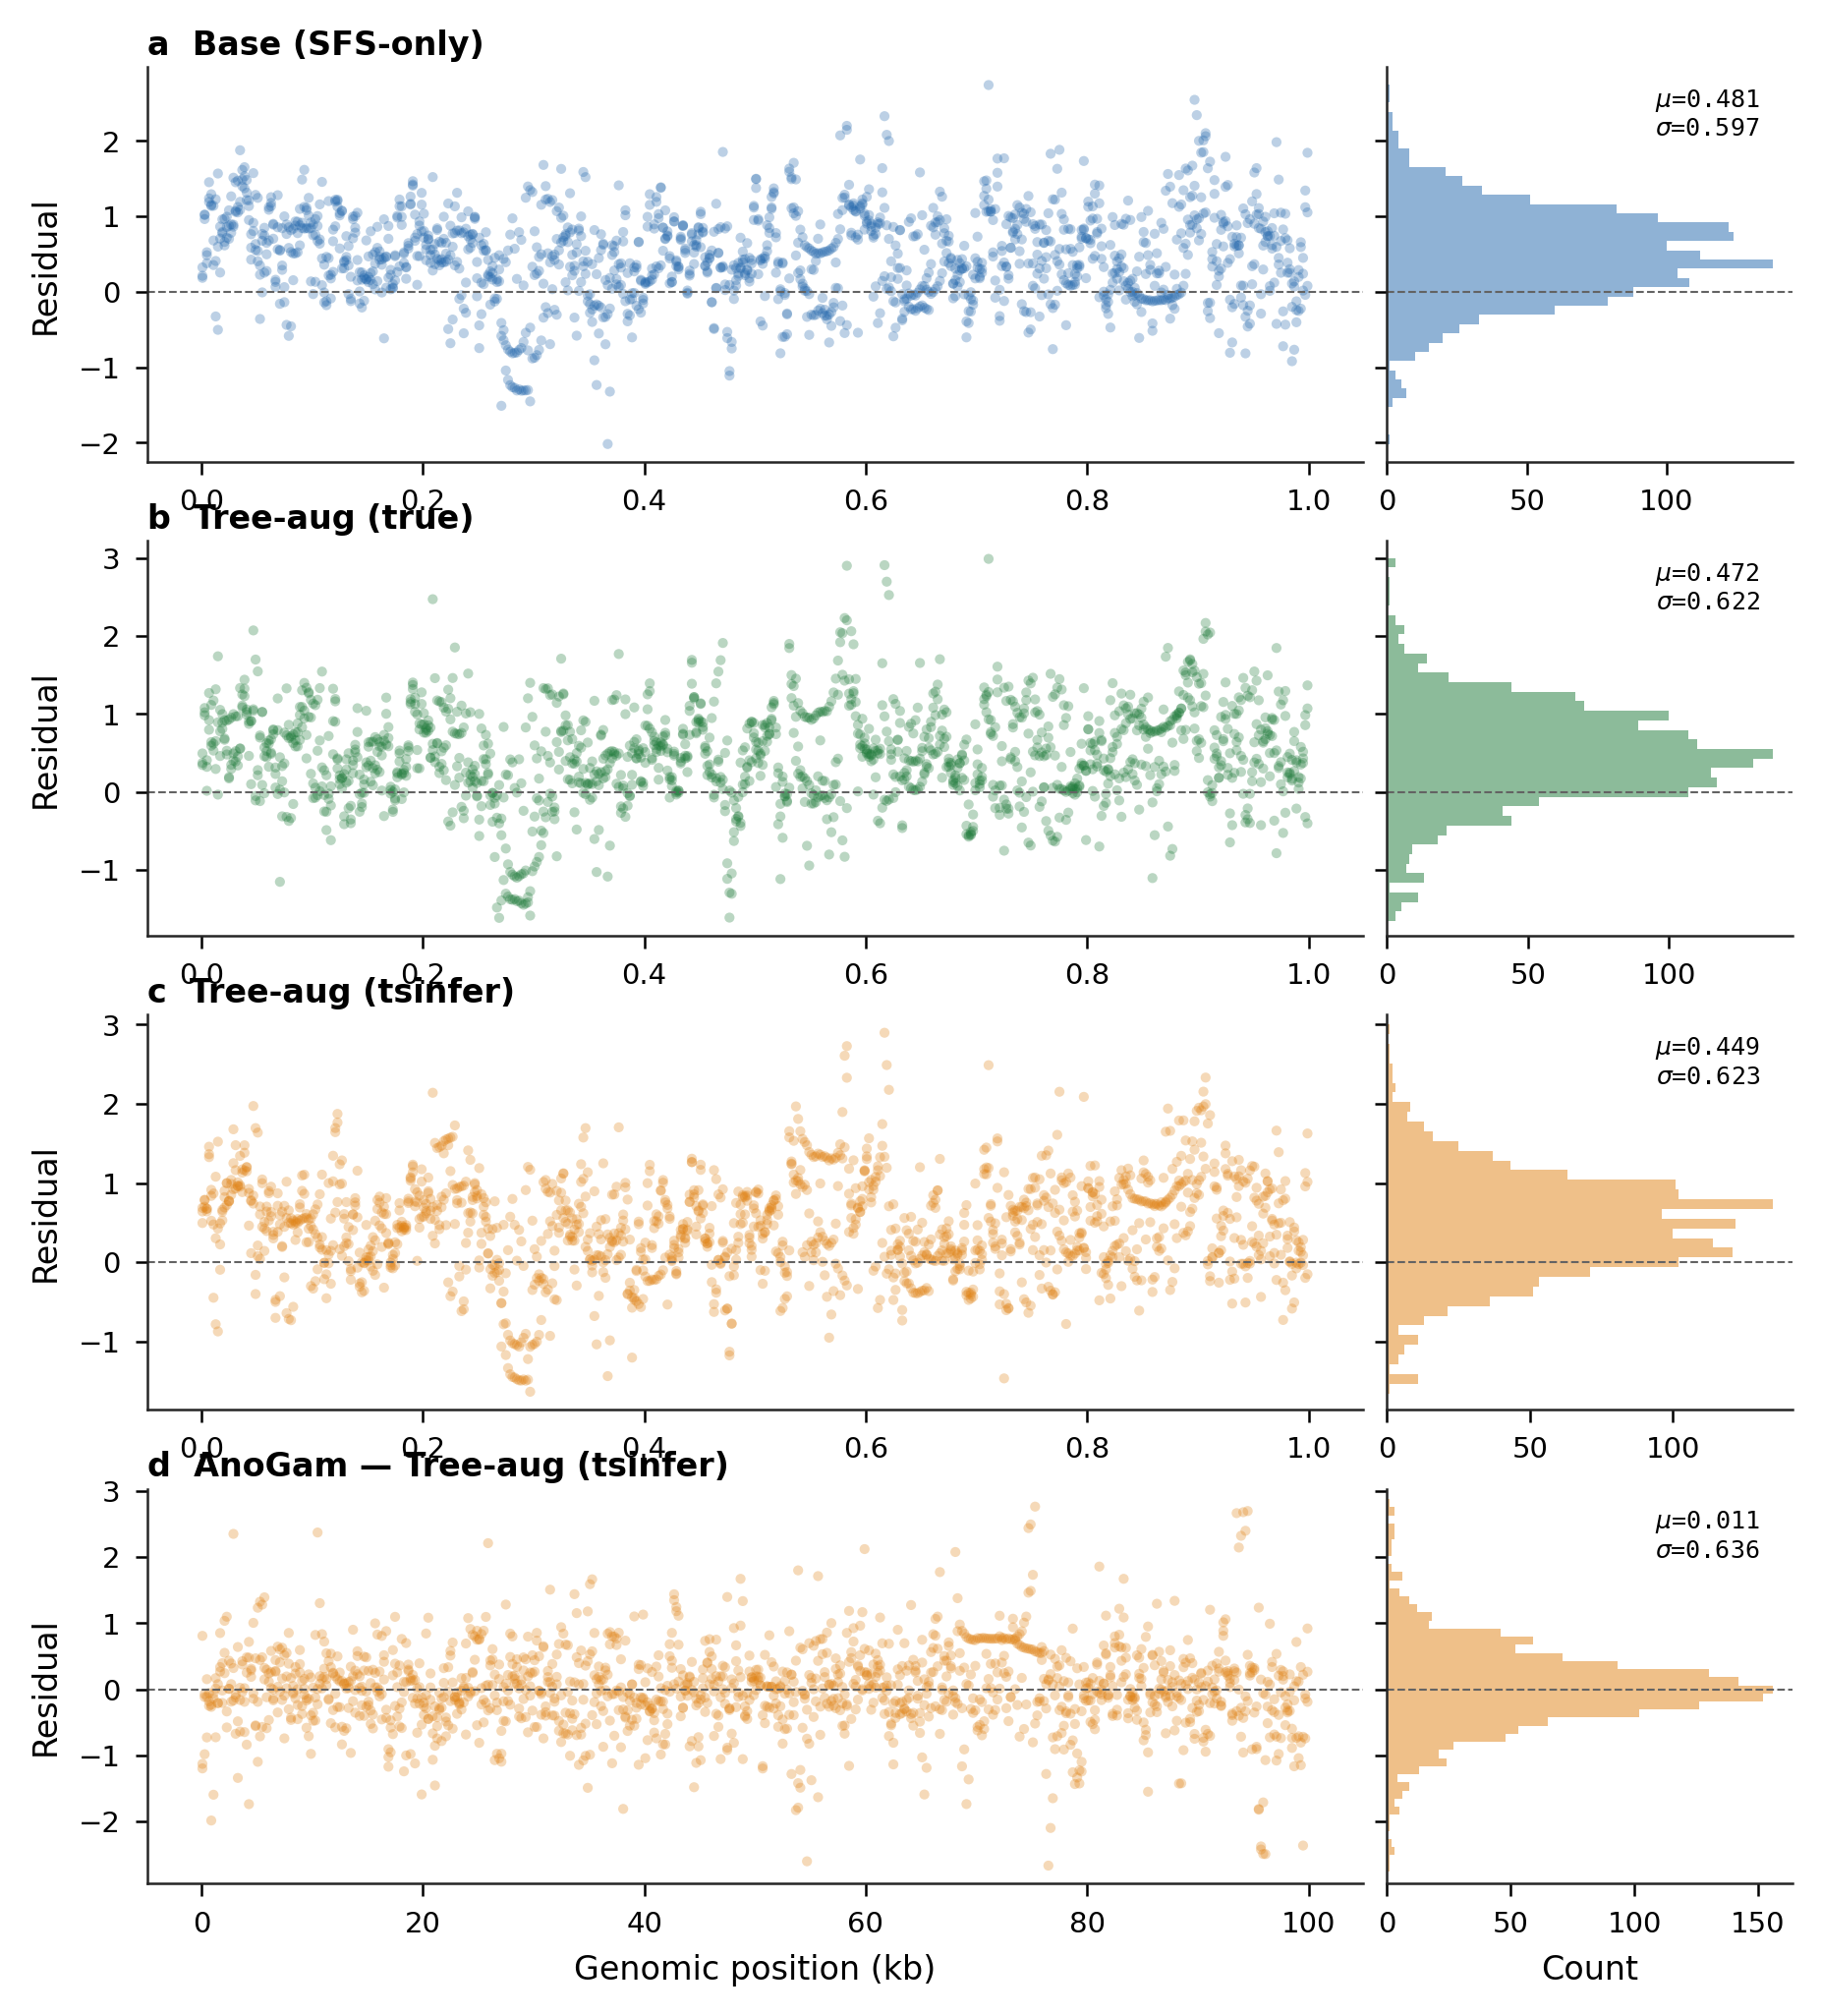
\includegraphics[width=\textwidth]{figS2_combined.png}\\[2pt]
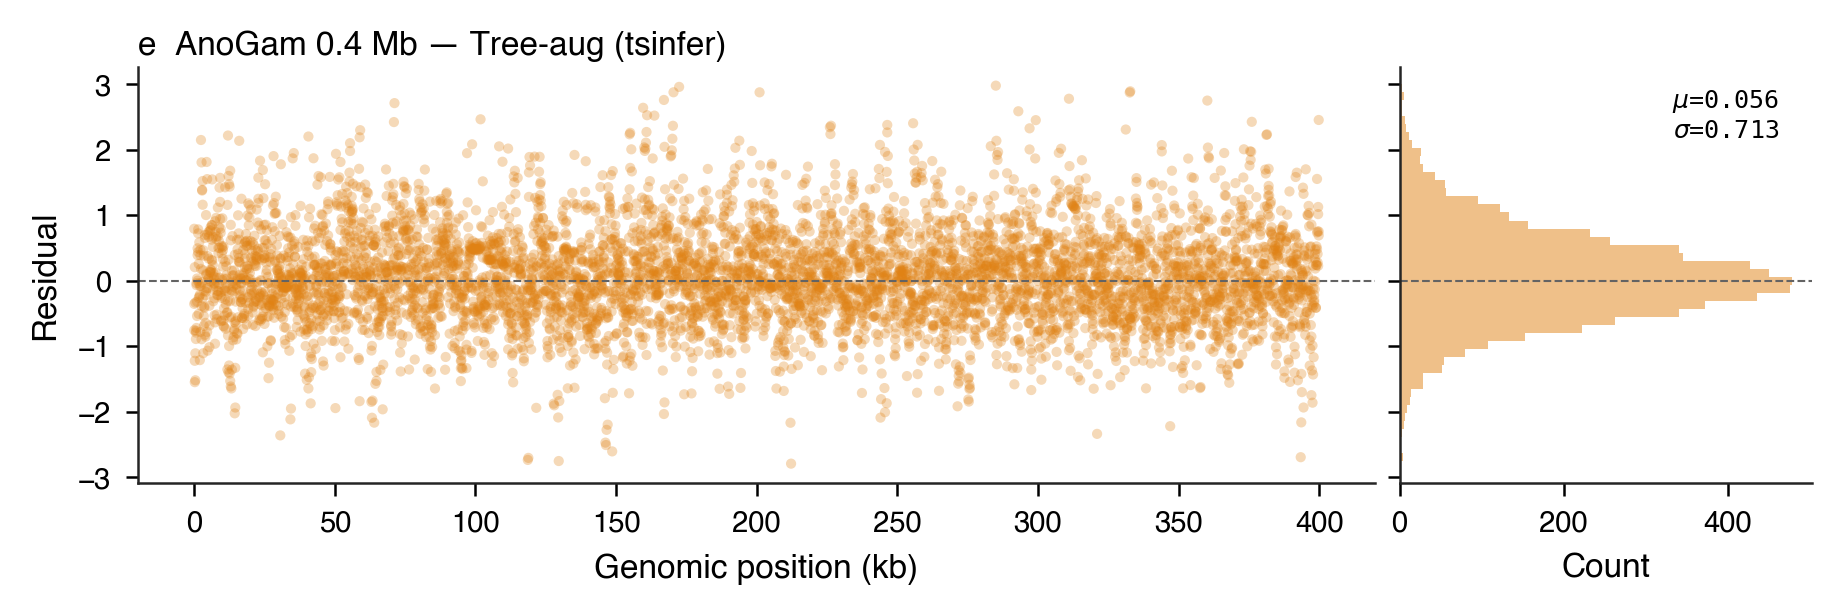
\includegraphics[width=\textwidth]{figS2e_residual_400kb.png}
\caption{Prediction residuals (predicted $-$ true) along the genome (left) and histograms
(right). (a)~Base (SFS-only), (b)~tree-aug (true), (c)~tree-aug (tsinfer)---all on
human-like 1\,Mb; (d)~AnoGam tree-aug (tsinfer, 100\,kb); (e)~AnoGam tree-aug (tsinfer,
400\,kb, 2{,}000 windows). Mean and standard deviation annotated in each panel.
All models show approximately centered, symmetric residuals with no spatial bias.}
\label{fig:residuals}
\end{figure}

\end{document}
